\documentclass[letterpaper,11pt]{article}

% --- PAQUETES DE IDIOMA
\usepackage[spanish,mexico]{babel}
\usepackage[utf8]{inputenc}
\usepackage{csquotes}
\usepackage[backend=biber,style=apa]{biblatex}
\DeclareLanguageMapping{spanish}{spanish-apa}
\addbibresource{referencias.bib}
\usepackage{iftex}

\usepackage{pdfpages}

% --- PAQUETES MATEMÁTICOS --
\usepackage{amsmath}
\usepackage{cancel}
\usepackage{mathrsfs}

% --- PAQUETES GRÁFICOS Y DE DISEÑO ---
\usepackage{graphicx}
\newcommand{\includegraphicssafe}[2] {%
  \IfFileExists{#2}{\includegraphics[width=#1]{#2}}{%
    \fbox{\parbox[c][4cm][c]{#1}{\centering Figura pendiente: \texttt{\detokenize{#2}}}}%
  }%
}
\usepackage{float}
\usepackage{placeins}
\usepackage{subcaption}
\usepackage[table]{xcolor}
\usepackage{makecell}
\usepackage{array}
\usepackage{longtable}
\usepackage{tabularx}
\newcolumntype{Y}{>{\raggedright\arraybackslash}X}
\usepackage{booktabs}
\newcolumntype{L}[1]{>{\raggedright\arraybackslash}p{#1}}
\usepackage{tikz}
\usetikzlibrary{shapes.geometric, shapes.multipart, positioning, arrows.meta, calc, shadows, decorations.pathreplacing,babel}

% --- LISTAS ---
\usepackage{enumitem}

% --- PAQUETES DE CÓDIGO ---
\usepackage{listings}
% Configuración del estilo de listings
\definecolor{codebg}{rgb}{0.95,0.95,0.95}   
\definecolor{keyword}{rgb}{0.0,0.2,0.6}     
\definecolor{comment}{rgb}{0.25,0.5,0.35}   
\definecolor{string}{rgb}{0.6,0.0,0.0}      
\definecolor{number}{rgb}{0.5,0.0,0.5}      
\definecolor{codegray}{rgb}{0.5,0.5,0.5}
\definecolor{codepurple}{rgb}{0.58,0,0.82}
\definecolor{backcolour}{rgb}{0.95,0.95,0.95}

\lstset{
  backgroundcolor=\color{backcolour},
  basicstyle=\ttfamily\small,
  keywordstyle=\color{blue}\bfseries,
  stringstyle=\color{codepurple},
  commentstyle=\color{codegray}\itshape,
  numbers=left,
  numberstyle=\tiny\color{codegray},
  frame=single,
  rulecolor=\color{black},
  breaklines=true,
  tabsize=4,
  showstringspaces=false,
  literate={á}{{\'a}}1
           {é}{{\'e}}1
           {í}{{\'i}}1
           {ó}{{\'o}}1
           {ú}{{\'u}}1
           {Á}{{\'A}}1
           {É}{{\'E}}1
           {Í}{{\'I}}1
           {Ó}{{\'O}}1
           {Ú}{{\'U}}1
           {ñ}{{\~n}}1
           {Ñ}{{\~N}}1
           {¿}{{\textquestiondown}}1
           {¡}{{\textexclamdown}}1
}

% Estilo para código en C
\lstdefinestyle{cstyle}{
  language=C,
  backgroundcolor=\color{backcolour},
  basicstyle=\ttfamily\small,
  keywordstyle=\color{blue}\bfseries,
    keywordstyle= \color{yellow!70!orange}\bfseries,
    morekeywords= {MPI_Init,MPI_Comm_size,MPI_Comm_rank,MPI_Send,MPI_Recv,MPI_Scatter,MPI_Gather,MPI_Bcast,MPI_Reduce,MPI_Finalize},
    emph={printf},
    emphstyle=\color{blue}\bfseries,
  stringstyle=\color{codepurple},
  commentstyle=\color{codegray}\itshape,
  numbers=left,
  numberstyle=\tiny\color{codegray},
  frame=single,
  rulecolor=\color{black},
  breaklines=true,
  tabsize=4,
  showstringspaces=false
}

% Definición del lenguaje Python para listings
\lstdefinelanguage[LAB]{Python}{
    morekeywords={False, None, True, and, as, assert, async, await, break,
                                class, continue, def, del, elif, else, except, finally,
                                for, from, global, if, import, in, is, lambda, nonlocal,
                                not, or, pass, raise, return, try, while, with, yield,
                                machine, Pin, PWM, ADC, Timer, sleep_ms, sleep_us},
    morecomment=[l]{\#},
    morestring=[b]",
    morestring=[b]',
    sensitive=true
}

% Estilo para salidas de consola/terminal
\lstdefinestyle{output}{
  backgroundcolor=\color{black!5},
  basicstyle=\ttfamily\footnotesize,
  numbers=none,
  frame=single,
  rulecolor=\color{black!30},
  breaklines=true,
  tabsize=4,
  showstringspaces=false,
  xleftmargin=0.5cm,
  xrightmargin=0.5cm
}

% --- ESTILOS PARA DIAGRAMAS DE FLUJO (TIKZ) ---
\tikzset{
  startstop/.style={rectangle, rounded corners, minimum width=3cm, minimum height=1cm,text centered, draw=black, fill=red!30},
  process/.style={rectangle, minimum width=3cm, minimum height=1cm, text centered, draw=black, fill=orange!30},
  decision/.style={diamond, aspect=2, minimum width=3cm, minimum height=1cm, text centered, draw=black, fill=green!30},
  io/.style={trapezium, trapezium left angle=70, trapezium right angle=110, minimum width=3cm, minimum height=1cm, text centered, draw=black, fill=blue!30},
  arrow/.style={thick,->,>=stealth}
}


\definecolor{azulresultado}{HTML}{0072C6}
\definecolor{rojoacarreo}{HTML}{FF0000}

% --- RUTAS DE IMÁGENES ---
\graphicspath{{img/}{portada_img/}}

\definecolor{armblue}{RGB}{0, 113, 188}

% --- ÍNDICE CON PUNTOS ---
\usepackage{tocloft}
\renewcommand{\cftsecleader}{\cftdotfill{\cftdotsep}}

% --- CONFIGURACIÓN DE PÁGINA (GEOMETRÍA) ---
\usepackage[
    left=25mm, 
    right=25mm,
    top=35mm,
    bottom=30mm,
    headheight=77pt, 
    papersize={21.59cm,27.94cm}
]{geometry}

% --- FORMATO DE TEXTO ---
\usepackage{setspace}
\onehalfspacing
\usepackage{parskip} 
\usepackage{lipsum}  

% --- VARIABLES GLOBALES ---
\newcommand{\materia}{}

% --- ENCABEZADOS Y PIES DE PÁGINA ---
\usepackage{fancyhdr}
\pagestyle{fancy}
\fancyhf{} 
\fancyhead[L]{
\includegraphics[height=1.5cm]{portada_img/der.png}}
\fancyhead[R]{
\includegraphics[height=1.5cm]{portada_img/izq.png}}
\fancyfoot[C]{\thepage} 
\renewcommand{\headrulewidth}{0.4pt} 
\renewcommand{\footrulewidth}{0pt}  

\fancypagestyle{indice}{
  \fancyhf{}
  \fancyhead[L]{
\includegraphics[height=1.5cm]{portada_img/der.png}}
  \fancyhead[R]{
\includegraphics[height=1.5cm]{portada_img/izq.png}}
  \fancyfoot{}
  \renewcommand{\headrulewidth}{0.4pt}
  \renewcommand{\footrulewidth}{0pt}
}

\fancypagestyle{referencias}{
  \fancyhf{}
  \fancyhead[L]{
\includegraphics[height=1.5cm]{portada_img/der.png}}
  \fancyhead[R]{
\includegraphics[height=1.5cm]{portada_img/izq.png}}
  \renewcommand{\headrulewidth}{0.4pt}
  \renewcommand{\footrulewidth}{0pt}
}

% --- HIPERVÍNCULOS ---
\usepackage{hyperref}
\hypersetup{
    colorlinks=true,
    linkcolor=blue,
    citecolor=blue,
    filecolor=magenta,
    urlcolor=cyan
}

\usepackage{caption}\captionsetup[table]{skip=8pt}
\begin{document}
\hypersetup{pageanchor=false}
\begin{titlepage}\thispagestyle{empty} % Sin encabezado ni pie en la portada

% --- ENCABEZADO DE PORTADA (TABLA DE 3 COLUMNAS) ---
\begin{center}
    % La tabla usa 'm' para centrar verticalmente las imagenes y el texto
    \begin{tabular}{m{0.15\textwidth} m{0.60\textwidth} m{0.15\textwidth}}
        % Logo Izquierdo (UNAM)
        
\includegraphics[width=2cm]{portada_img/der.png} & 
        
        % Titulo Central
        \centering\LARGE\textbf{Universidad Nacional Autonoma de Mexico} &
        
        % Logo Derecho (Facultad)
        \raggedleft
\includegraphics[width=2cm]{portada_img/izq.png}
    \end{tabular}
\end{center}

\vspace{0.3cm}

% --- INFORMACION DEL REPORTE ---
\begin{center}
    {\LARGE \textbf{Facultad de Ingenieria}}\\[0.45cm]

    {\LARGE \textbf{Alumno:}}\\[0.3cm]
    {\Large Lara Hernandez Angel Husiel - 320060829} \\[0.45cm]
    {\Large Lugo Manzano Rodrigo - 320206968} \\[0.45cm]
    {\Large Garcia Cortes Adolfo de Jesus - 320317264} \\[0.45cm]


    {\LARGE \textbf{Mineria de datos.}} \\[0.45cm]

	{\LARGE Grupo: 01 - Semestre: 2027-1} \\[0.45cm]
    
    {\LARGE \textbf{Proyecto final}}\\[0.5cm]

    {\LARGE {Analisis de recepcion y popularidad de videojuegos mediante mineria de datos}}\\[0.45cm]

    {\LARGE \textbf{Profesor:}}\\[0.2cm]
    {\Large MTRO. GERARDO GABRIEL CARRASCO ZUÑIGA}\\[0.45cm]

    {\Large \textbf{Fecha de corte:}}\\[0.2cm]
    {\Large 12 de noviembre de 2026}
\end{center}\end{titlepage}
\newpage
{\makeatletter\let\ps@plain\ps@indice\makeatother
\pagestyle{indice}\thispagestyle{indice}\hypersetup{linkcolor=black}\tableofcontents\thispagestyle{indice}}
\newpage\setcounter{page}{1}\hypersetup{pageanchor=true}\singlespacing
\section*{Resumen}\addcontentsline{toc}{section}{Resumen}
Este proyecto tiene como finalidad analizar de forma práctica cómo se relacionan la opinión de los jugadores, la crítica especializada y la popularidad que alcanza un videojuego dentro de Backloggd. La idea surge porque normalmente se utiliza una calificación para hablar del éxito de un título, aunque esa nota no nos dice cuántas personas lo juegan ni cuántas tienen interés en hacerlo. Para atender esta situación se revisaron las calificaciones y las métricas de interacción por separado, después se buscaron grupos de juegos similares y finalmente se construyó una aplicación que permite consultar los resultados y probar un modelo supervisado.

El original designado, \texttt{games\_curated.csv}, contiene 1,117 registros y 42 columnas; 1,114 son elegibles para el análisis principal y 887 tienen las seis variables completas para clustering. Pearson entre usuarios y prensa es 0.5439 en esos 887 pares. K-Means con dos grupos alcanza silhouette de 0.3188 en Python. El Random Forest de la web obtiene 56.76\,\% de exactitud y F1 macro de 0.5577 sobre 222 casos de prueba. En Weka, RandomForest obtiene 53.4753\,\% con validación cruzada de diez pliegues sobre 892 registros exportados. Las evaluaciones no son equivalentes y se presentan por separado.

La aplicación permite explorar los hallazgos, enviar atributos crudos al Pipeline y consultar vecinos del entrenamiento. El resultado más importante es que podemos describir diferencias de recepción y popularidad dentro del catálogo, pero no demostrar rentabilidad, causalidad ni riesgo financiero de juegos como servicio. La clase media y la cobertura de prensa limitan la utilidad predictiva.

\section{Objetivos del proyecto}\label{sec:objetivos}
\subsection{Objetivo general}
Aplicar técnicas de minería de datos sobre el catálogo de videojuegos contenido en games\_curated.csv para analizar la diferencia entre la valoración de la comunidad y la crítica especializada, reconocer cómo se distribuyen la actividad y el interés de los jugadores, encontrar grupos de títulos con características similares y estimar su nivel de popularidad relativa mediante un modelo supervisado. Los resultados se integran en una aplicación web local para que puedan explorarse y contrastarse con ejemplos concretos.
\subsection{Objetivos específicos}
\begin{enumerate}
\item Verificar el esquema, las escalas, los faltantes y la procedencia del maestro, conservando su integridad y documentando cada transformación.
\item Estimar Pearson y Spearman entre notas, reportando tamaño muestral y p-valor por catálogo, género y organización, con un mínimo de veinte pares completos por grupo.
\item Describir Plays, Playing, Backlogs y Wishlist; distinguir actividad observada de interés pendiente sin equipararlas a ventas.
\item Comparar K-Means de dos a diez grupos y DBSCAN sobre seis variables transformadas, informando silhouette cuando sea definida, tamaño, ruido y composición de los perfiles.
\item Comparar una referencia mayoritaria, Naive Bayes, árbol y bosque para clasificar terciles de popularidad con entradas que no incluyan las señales del objetivo.
\item Verificar el formulario contra el Pipeline guardado y ofrecer una demo local con exploración, predicción y explicación de las limitaciones.
\end{enumerate}
\subsection{Expectativas y criterios de aceptación}
Esperábamos encontrar relaciones entre las notas, perfiles interpretables y un clasificador superior a una referencia mayoritaria. Estas expectativas se comprueban con evidencia, no por la apariencia de las gráficas. Una correlación no equivale a acuerdo; un grupo dominante no basta para afirmar segmentación útil; una exactitud superior al azar no garantiza buen desempeño en cada clase.

El proyecto se considera funcional cuando las tablas y predicciones se reproducen, las transformaciones no usan información de prueba y la aplicación muestra los resultados del artefacto real. La capacidad para predecir éxito comercial queda fuera del criterio de aceptación porque no puede verificarse con este archivo.
\section{Contexto del proyecto}\label{sec:contexto}
\subsection{Origen y unidad de análisis}
El antecedente se atribuye al conjunto de Arnab Chaki publicado en Kaggle, construido con información de Backloggd \parencite{chaki2023popular}. El archivo que el usuario designó como original es una versión ya curada, no una descarga virgen del catálogo público. Contiene datos adicionales, incluidas notas y estimaciones. La portada del dataset menciona 1980--2023, pero el maestro local tiene cobertura histórica hasta 2025; no sustituimos una cosa por la otra.

La unidad analítica se identifica por \texttt{id\_juego}. El mismo título puede aparecer con otra fecha, por lo que las uniones no se realizan solo por nombre. Hay 35 registros de 17 títulos repetidos en fechas distintas. Para particionar el modelo sí agrupamos nombres normalizados, de forma conservadora, para que versiones del mismo título no aparezcan a ambos lados de la evaluación.
\subsection{Variables y escalas verificadas}
Rating corresponde a usuarios en escala de cero a cinco; su rango observado es 0.7 a 4.8, con trece ausencias. La nota original de Metacritic tiene valores de 45 a 99; la escala de referencia de prensa es cero a cien. Los extremos observados no se usan como denominadores de normalización.

Plays representa registros de juego; Playing contextualiza actividad en curso; Backlogs y Wishlist reflejan interés registrado. No son personas únicas verificadas, copias vendidas ni ingresos. Genres y Team son listas. Team puede mezclar organizaciones con papeles distintos y no acredita por sí mismo cuál desarrolló o publicó el juego.

El maestro incluye columnas financieras estimadas. No se utilizan para concluir que un título fue rentable. Asimismo, 218 notas marcadas como estimaciones propias no se aceptan como evidencia independiente de prensa: en el antecedente, 214 estimaciones con Rating siguen una relación lineal tras redondear. Incluirlas inflaría artificialmente la relación que se desea estudiar.
\subsection{Poblaciones y sesgos}
El antecedente de 1,512 registros se reconstruye hasta el maestro de 1,117, con 395 descartes históricos documentados. Esto no significa que la limpieza actual haya eliminado 395 filas: recibe un maestro ya curado y conserva sus 1,117 registros. Tres conflictos históricos se mantienen señalados y se excluyen del análisis principal; quedan 1,114 elegibles.

Las correlaciones y el clustering completo usan 887 casos elegibles con las notas y señales necesarias. Las ausencias no son ruido de DBSCAN ni una categoría de popularidad. La selección de juegos visibles en Backloggd implica sesgo de cobertura y supervivencia; las conclusiones se limitan al catálogo y al corte disponible.
\section{Estrategia a seguir}\label{sec:estrategia}
Adoptamos CRISP-DM como estructura de trabajo \parencite{chapman2000crisp}. Sus seis fases organizan la comprensión del problema, la inspección, la preparación, el modelado, la evaluación y la entrega. No las confundimos con los nombres de scripts: \texttt{03\_clustering.py} corresponde a tareas de modelado y evaluación, no a una tercera fase de negocio.

El proceso fue iterativo. Las auditorías obligaron a revisar la procedencia de las notas, la definición del objetivo y las separaciones del entrenamiento. La propuesta propia en Python consiste en integrar estas salvaguardas en Pipelines, recalcular referencias del objetivo dentro de cada pliegue y verificar la inferencia del formulario. La complejidad adicional no se justifica por agregar un modelo más, sino por evitar que una comparación favorable provenga de fuga de información.

Las herramientas cumplen papeles distintos: pandas prepara y verifica tablas; matplotlib produce figuras de reporte; scikit-learn entrena y evalúa; Weka aporta corridas gráficas de una herramienta de la materia; Streamlit y Plotly presentan resultados interactivos; LaTeX integra la documentación. El uso del Pipeline facilita mantener el mismo preprocesamiento en validación e inferencia \parencite{pedregosa2011scikit,sklearncv}.
\section{Problemática a atender}
La problemática principal es que el éxito de un videojuego no se puede explicar con un solo indicador. Por ejemplo, un título puede tener una calificación alta porque quienes lo jugaron quedaron satisfechos, pero eso no significa que haya llegado a una comunidad numerosa. También puede suceder lo contrario: un juego conocido puede acumular muchos registros de actividad y al mismo tiempo recibir opiniones divididas. Si únicamente revisamos la nota, estaríamos dejando fuera una parte importante de lo que sucede con ese videojuego.

La preocupación del anteproyecto por las apuestas a géneros y juegos como servicio sirvió para plantear el problema. Sin embargo, los datos no contienen una identificación confiable de GaaS ni ingresos, costos y ventas observados. Por ello no atribuimos fracasos comerciales a la elección de un género ni presentamos el modelo como una herramienta para evitar pérdidas. Esa relación requeriría otras fuentes y otro diseño de estudio.

Por esta razón, el proyecto se concentró en utilizar los datos que sí teníamos disponibles: las opiniones, los registros de juego y las listas de interés. Esto nos permite comparar situaciones diferentes dentro del catálogo y revisar si un modelo puede reconocerlas a partir del género, la organización, la década y las calificaciones. El resultado puede servir para orientar una exploración del mercado, aunque por sí solo no reemplaza un estudio de ventas o rentabilidad.
\section{Preparación y control de calidad}\label{sec:preparacion}
Los campos numéricos se interpretan con una función que reconoce sufijos K y M, espacios y nulos; un texto inválido no se convierte silenciosamente a cero. No obstante, los seis conteos del maestro ya eran numéricos: la limpieza actual no se adjudica conversiones que no realizó. Las pruebas sí incluyen casos como 999, 1K y 1.5M.

Las fechas se convierten a un formato común y generan año y década. Se mantienen tres fechas ausentes con sus indicadores en lugar de inventarlas. Los géneros se conservan como listas y se expanden a una tabla larga de 2,682 pertenencias. El género principal es una convención de presentación, no una taxonomía dominante demostrada; un juego participa en cada género declarado cuando hacemos análisis por género.

Una decisión importante fue no llenar las calificaciones faltantes durante el análisis descriptivo. Si asignábamos una nota promedio antes de comparar usuarios y prensa, estaríamos agregando información que no estaba realmente en el archivo. Por eso las correlaciones utilizan únicamente los pares disponibles. La mediana se utiliza después, cuando el modelo necesita una entrada completa, y se calcula solamente con los datos de entrenamiento. De la misma forma, las notas marcadas como estimaciones propias no se tratan como una opinión independiente de la prensa.

La normalización y la brecha se definen como:
\begin{equation} R_{100}=\frac{R}{5}\,100,\qquad \Delta=R_{100}-M.\end{equation}
Un signo positivo indica que la valoración de usuarios normalizada es mayor. La brecha absoluta mide distancia entre puntuaciones, mientras que Pearson mide asociación. No aplicamos min--max con los extremos de la muestra porque cambiaría el significado de la brecha cada vez que cambia el catálogo.

La limpieza registra conteos antes y después de cada paso y conserva el maestro. Los indicadores de conflicto y elegibilidad permiten conservar filas para trazabilidad sin introducirlas en la evaluación principal. Los hashes aportan una comprobación adicional de integridad, pero no garantizan que la fuente histórica carezca de errores.
\section{Análisis exploratorio y recepción}\label{sec:eda}
\subsection{Actividad e interés}
La distribución de actividad e interés es asimétrica. Por eso presentamos conteos con escala logarítmica para que los títulos de menor alcance no desaparezcan frente a los más conocidos. Logaritmar la visualización no crea popularidad nueva ni cambia el orden de los juegos.

Plays se interpreta como alcance registrado y Backlogs y Wishlist como interés pendiente. Playing se conserva como contexto de actividad. Esto quiere decir que aparecer en muchas listas no garantiza que esas personas finalmente jueguen el título. El interés pendiente y la actividad ya registrada nos hablan de momentos distintos. Por eso un índice alto se interpreta como una posición alta dentro del catálogo y no como una cantidad de ventas.

\begin{figure}[htbp]\centering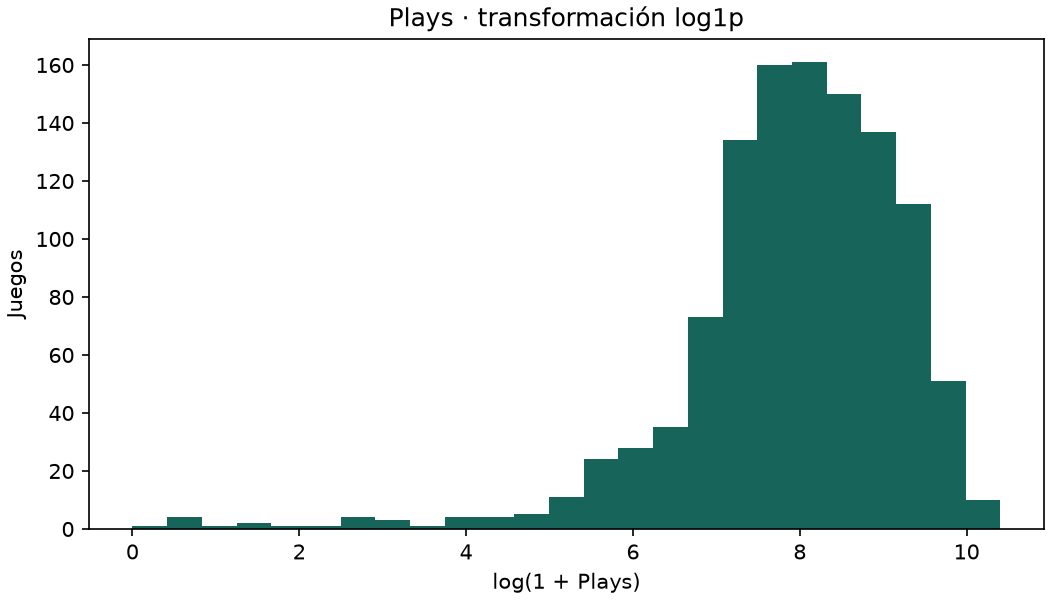
\includegraphics[width=\linewidth,height=.42\textheight,keepaspectratio]{figuras/eda_plays_log.png}
\caption{Distribución de Plays en la inspección del maestro. Fuente: figura reproducible del proyecto.}\end{figure}\FloatBarrier

\begin{figure}[htbp]\centering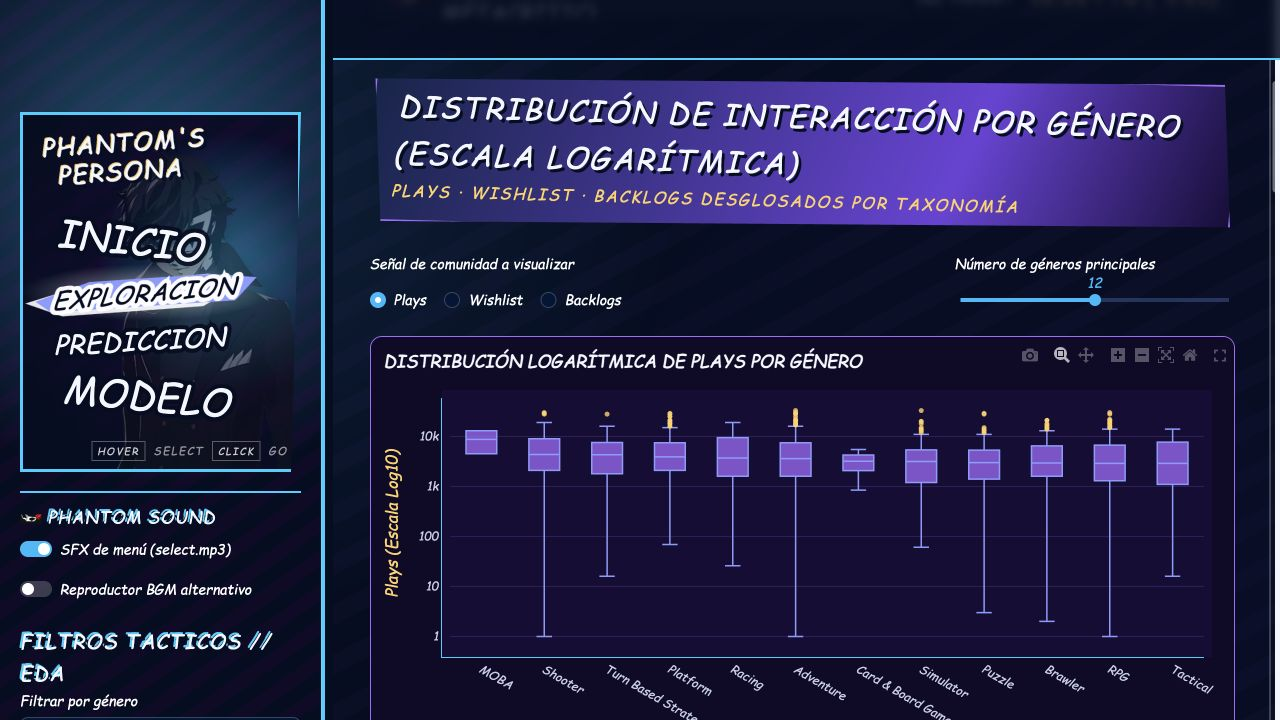
\includegraphics[width=\linewidth,height=.48\textheight,keepaspectratio]{figuras/graficas_logaritmicas_corregidas.jpg}
\caption{Distribución de interacción por género en la aplicación. Escala logarítmica y etiquetas mayores legibles.}\end{figure}\FloatBarrier

\begin{longtable}{p{0.174\textwidth}p{0.174\textwidth}p{0.174\textwidth}p{0.174\textwidth}p{0.174\textwidth}}
\caption{Relaciones de rango entre señales y notas; pares completos para cada comparación. Un p impreso como cero corresponde al límite numérico del cálculo, no a una probabilidad matemática exactamente nula.}\\
\toprule
Variable A & Variable B & Pares & Spearman & p Spearman\\\midrule\endfirsthead
Variable A & Variable B & Pares & Spearman & p Spearman\\\midrule\endhead
Plays & Playing & 1114 & 0.5471 & 5.44e-88\\
Plays & Backlogs & 1114 & 0.5973 & 1.15e-108\\
Plays & Wishlist & 1114 & 0.3413 & 8.70e-32\\
Plays & Rating & 1101 & 0.0874 & 3.72e-03\\
Plays & Metacritic Rating & 896 & 0.4230 & 3.29e-40\\
Playing & Backlogs & 1114 & 0.7505 & 3.14e-202\\
Playing & Wishlist & 1114 & 0.7013 & 1.13e-165\\
Playing & Rating & 1101 & 0.4017 & 5.98e-44\\
Playing & Metacritic Rating & 896 & 0.3458 & 1.45e-26\\
Backlogs & Wishlist & 1114 & 0.8542 & 0.00e+00\\
Backlogs & Rating & 1101 & 0.4133 & 1.14e-46\\
Backlogs & Metacritic Rating & 896 & 0.4330 & 3.10e-42\\
Wishlist & Rating & 1101 & 0.5035 & 7.76e-72\\
Wishlist & Metacritic Rating & 896 & 0.3698 & 2.04e-30\\
Rating & Metacritic Rating & 887 & 0.5242 & 9.34e-64\\
\bottomrule\end{longtable}

\subsection{Usuarios y prensa}
En el catálogo elegible, Pearson es 0.5439 con $p=1.936\times10^{-69}$ y Spearman es 0.5242 con $p=9.34\times10^{-64}$, sobre 887 pares completos. La asociación positiva es moderada; el p-valor pequeño no transforma esa asociación en acuerdo perfecto ni en efecto causal.

Para grupos se exige un mínimo de veinte pares válidos, no simplemente veinte filas. Los géneros se superponen: sus tamaños no deben sumarse para obtener el total de juegos. Los estudios se presentan como organizaciones de Team y no como desarrolladores confirmados. La comprobación con Spearman reduce la dependencia de una relación estrictamente lineal, pero tampoco demuestra acuerdo.

\begin{longtable}{p{0.174\textwidth}p{0.174\textwidth}p{0.174\textwidth}p{0.174\textwidth}p{0.174\textwidth}}
\caption{Correlaciones por género. La tabla conserva las filas reportadas; las exclusiones se documentan en la evidencia.}\\
\toprule
Género & Pares & Pearson & p Pearson & Spearman\\\midrule\endfirsthead
Género & Pares & Pearson & p Pearson & Spearman\\\midrule\endhead
Adventure & 598 & 0.5746 & 7.92e-54 & 0.5443\\
RPG & 286 & 0.5014 & 1.30e-19 & 0.5175\\
Shooter & 223 & 0.5596 & 8.89e-20 & 0.5286\\
Platform & 188 & 0.6428 & 2.68e-23 & 0.5525\\
Indie & 166 & 0.5383 & 7.45e-14 & 0.5536\\
Puzzle & 110 & 0.3601 & 1.12e-04 & 0.4500\\
Strategy & 94 & 0.4340 & 1.24e-05 & 0.3373\\
Brawler & 97 & 0.6160 & 1.87e-11 & 0.6150\\
Simulator & 79 & 0.5347 & 3.85e-07 & 0.5026\\
Turn Based Strategy & 51 & 0.2514 & 7.52e-02 & 0.3820\\
Fighting & 46 & 0.6188 & 4.58e-06 & 0.5826\\
Arcade & 39 & 0.7548 & 2.83e-08 & 0.6229\\
Visual Novel & 27 & -0.1042 & 6.05e-01 & -0.1382\\
Tactical & 37 & 0.3467 & 3.55e-02 & 0.3602\\
Racing & 31 & 0.4916 & 4.98e-03 & 0.4357\\
Point-and-Click & 27 & 0.6546 & 2.12e-04 & 0.6395\\
Music & 18 & No aplica & No aplica & No aplica\\
Sport & 18 & No aplica & No aplica & No aplica\\
Card \& Board Game & 10 & No aplica & No aplica & No aplica\\
Real Time Strategy & 9 & No aplica & No aplica & No aplica\\
Quiz/Trivia & 2 & No aplica & No aplica & No aplica\\
MOBA & 2 & No aplica & No aplica & No aplica\\
Pinball & 1 & No aplica & No aplica & No aplica\\
\bottomrule\end{longtable}

Los resultados no sostienen que todos los géneros tengan la misma relación. Arcade presenta $r=0.7548$ con 39 pares, mientras que Visual Novel tiene $r=-0.1042$ con 27 y $p=0.605$. En este último grupo no hay evidencia suficiente de asociación lineal distinta de cero. Comparar coeficientes de grupos superpuestos no constituye una prueba formal de diferencia entre géneros.

\begin{longtable}{p{0.217\textwidth}p{0.217\textwidth}p{0.217\textwidth}p{0.217\textwidth}}
\caption{Asociaciones de las primeras doce organizaciones reportadas, ordenadas por cobertura.}\\
\toprule
Organización & Pares & Pearson & p Pearson\\\midrule\endfirsthead
Organización & Pares & Pearson & p Pearson\\\midrule\endhead
Nintendo & 125 & 0.4410 & 2.64e-07\\
Capcom & 51 & 0.6717 & 6.80e-08\\
Square Enix & 49 & 0.5977 & 5.77e-06\\
Sega & 31 & 0.6937 & 1.51e-05\\
Electronic Arts & 42 & 0.5580 & 1.23e-04\\
Konami & 22 & 0.6180 & 2.17e-03\\
Activision & 26 & 0.4132 & 3.59e-02\\
Bandai Namco Entertainment & 25 & 0.7966 & 1.90e-06\\
Ubisoft Entertainment & 27 & 0.6419 & 3.08e-04\\
Atlus & 23 & 0.5554 & 5.93e-03\\
Sony Interactive Entertainment & 22 & 0.7309 & 1.12e-04\\
Nintendo EAD & 15 & No aplica & No aplica\\
\bottomrule\end{longtable}

\begin{longtable}{p{0.217\textwidth}p{0.217\textwidth}p{0.217\textwidth}p{0.217\textwidth}}
\caption{Orden de géneros por menor distancia absoluta media entre puntuaciones.}\\
\toprule
Género & Pares & Brecha absoluta & Pearson\\\midrule\endfirsthead
Género & Pares & Brecha absoluta & Pearson\\\midrule\endhead
Visual Novel & 27 & 8.2222 & -0.1042\\
Brawler & 97 & 8.9588 & 0.6160\\
Point-and-Click & 27 & 9.0000 & 0.6546\\
Arcade & 39 & 9.0513 & 0.7548\\
RPG & 286 & 9.3462 & 0.5014\\
Indie & 166 & 9.5422 & 0.5383\\
Turn Based Strategy & 51 & 9.5686 & 0.2514\\
Puzzle & 110 & 9.9818 & 0.3601\\
Adventure & 598 & 10.1070 & 0.5746\\
Simulator & 79 & 10.1646 & 0.5347\\
Platform & 188 & 10.5532 & 0.6428\\
Tactical & 37 & 11.0270 & 0.3467\\
Strategy & 94 & 11.8936 & 0.4340\\
Racing & 31 & 12.0000 & 0.4916\\
Fighting & 46 & 12.0217 & 0.6188\\
Shooter & 223 & 12.8206 & 0.5596\\
\bottomrule\end{longtable}

Visual Novel aparece con menor distancia media entre notas, pero su correlación no es positiva de forma concluyente. Esto muestra por qué distinguimos coincidencia de niveles y asociación: que dos series tengan notas cercanas no implica que ordenen los juegos de la misma forma. Los p-valores segmentados son exploratorios; el proyecto también conserva ajustes por comparaciones múltiples en las tablas originales.
\section{Clustering y perfiles del catálogo}\label{sec:clustering}
\subsection{Transformación y elección de K-Means}
Se utilizaron Plays, Playing, Backlogs, Wishlist, Rating y Metacritic Rating. Los cuatro conteos reciben $\log(1+x)$ y después se estandarizan las seis variables. Con ello reducimos la asimetría de los conteos y evitamos que las unidades de una sola variable dominen la distancia. El género no entra a la distancia; sirve para interpretar la composición posterior.

K-Means se evaluó de $k=2$ a $10$, con semilla 42 y treinta inicializaciones. La elección de dos grupos maximiza silhouette, 0.3188; los valores de $k=3$ y $k=4$ son 0.2377 y 0.2268. La inercia disminuye al aumentar grupos, por lo que no se usa su mínimo como una regla automática para escoger el mayor $k$.

\begin{figure}[htbp]\centering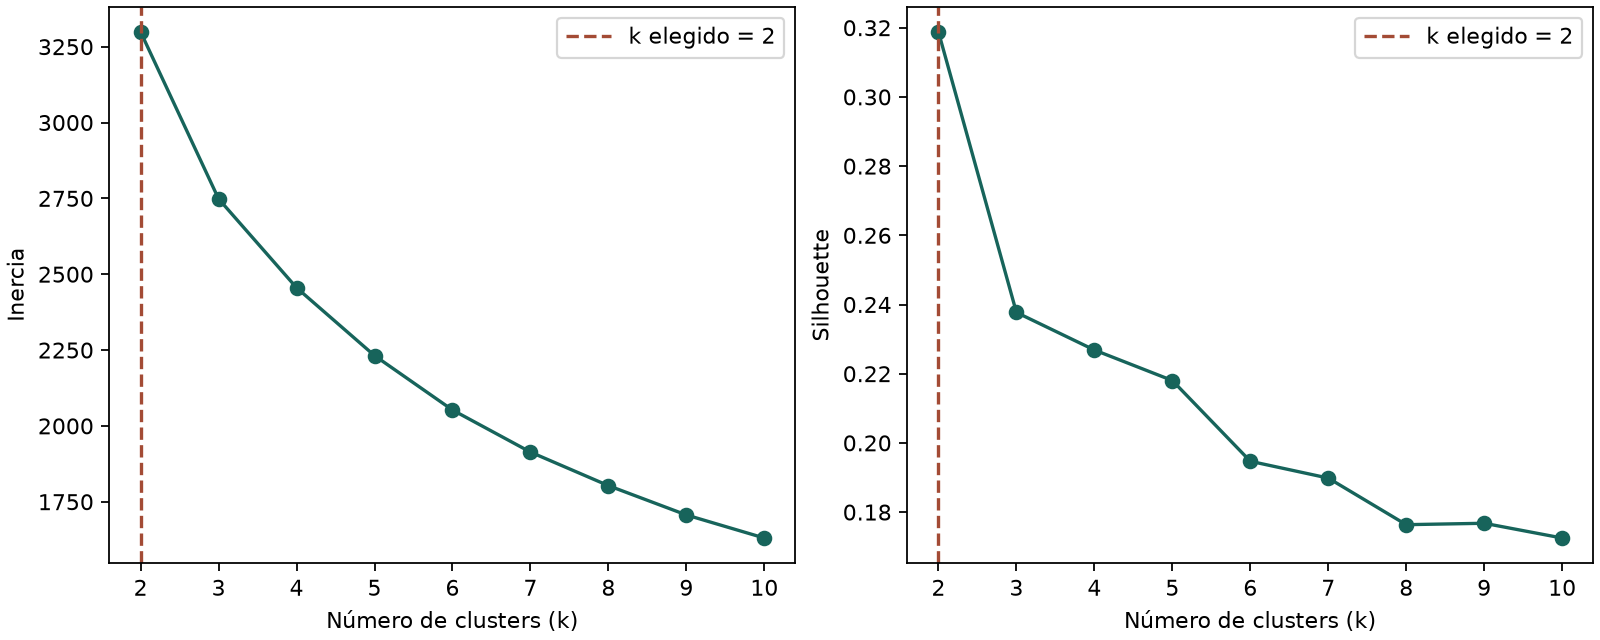
\includegraphics[width=\linewidth,height=.45\textheight,keepaspectratio]{figuras/clustering_03_kmeans.png}
\caption{Inercia y silhouette para la selección de k. Fuente: ejecución de Python.}\end{figure}\FloatBarrier

Los grupos de Python contienen 465 y 422 juegos. El primero combina mayor actividad, interés y notas medias: Plays 7,680.62, Wishlist 1,053.28 y Rating 3.91; el segundo registra Plays 2,980.68, Wishlist 246.23 y Rating 3.38. Los nombres propuestos describen esas diferencias y no certifican segmentos comerciales naturales.

Adventure aparece en ambos perfiles, por lo que su predominio no distingue por sí solo una oportunidad de mercado. Además, la primera separación resume magnitud conjunta: las alternativas con tres y cuatro grupos se conservaron para explorar combinaciones sin cambiar la selección por conveniencia narrativa. La figura PCA es una proyección descriptiva y no las dimensiones con las que se entrenó K-Means.

\begin{figure}[htbp]\centering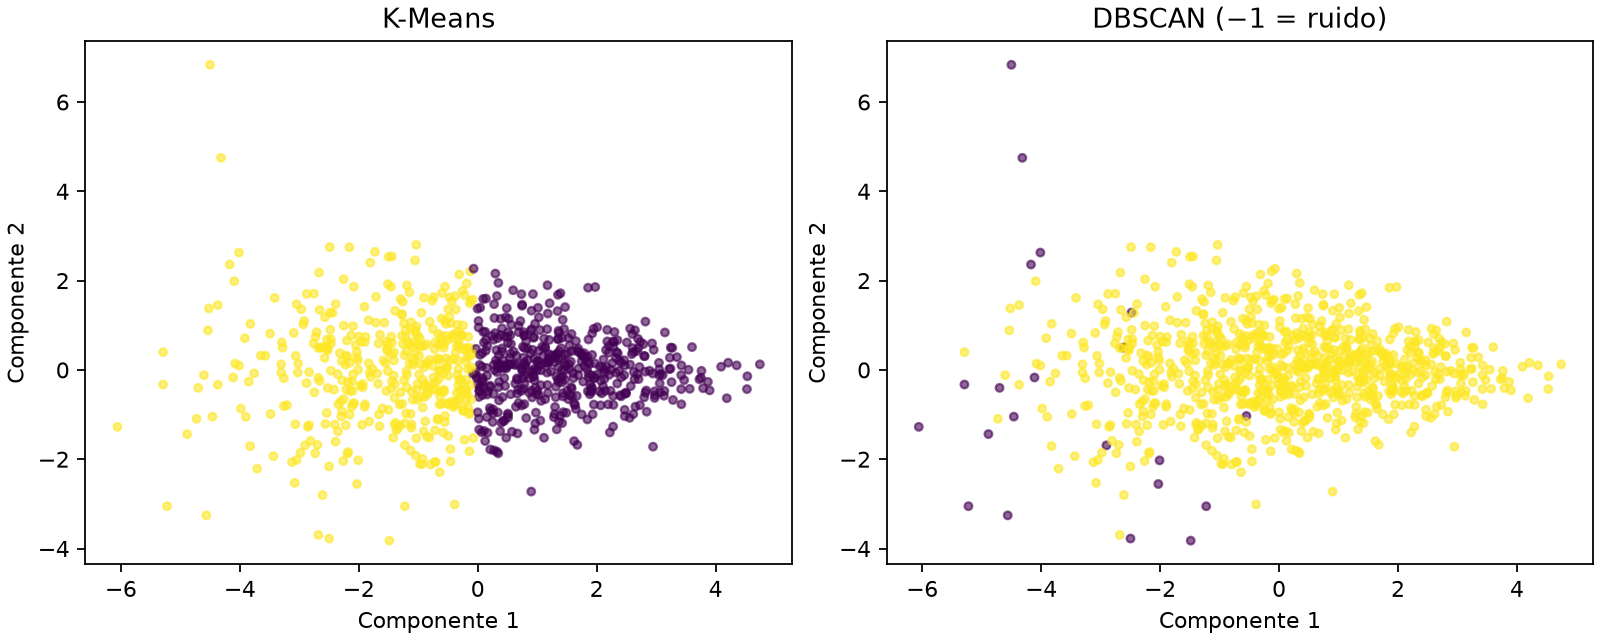
\includegraphics[width=\linewidth,height=.48\textheight,keepaspectratio]{figuras/clustering_03_proyeccion.png}
\caption{Proyección de los casos agrupables. Los ejes reducidos se utilizan para visualización, no para definir el objetivo supervisado.}\end{figure}\FloatBarrier

\begin{longtable}{p{0.29\textwidth}p{0.29\textwidth}p{0.29\textwidth}}
\caption{Cinco ejemplos descriptivos por grupo K-Means, próximos al centro del perfil en el espacio transformado.}\\
\toprule
Grupo & ID & Juego\\\midrule\endfirsthead
Grupo & ID & Juego\\\midrule\endhead
0 & 1056 & The Messenger\\
0 & 304 & Dragon Age: Origins\\
0 & 172 & Metroid: Zero Mission\\
0 & 980 & The Legend of Zelda: Majora's Mask 3D\\
0 & 517 & Luigi's Mansion 3\\
1 & 1360 & Sonic Rush Adventure\\
1 & 1420 & Black\\
1 & 1375 & Toy Story 2: Buzz Lightyear to the Rescue!\\
1 & 1398 & Shantae: Half-Genie Hero\\
1 & 1338 & Condemned: Criminal Origins\\
\bottomrule\end{longtable}

\subsection{DBSCAN y puntos atípicos}
La elección de eps usa la curva de distancia al vecino y una regla geométrica reproducible sobre la curva normalizada. Se obtuvo eps de 1.666296, con doce vecinos mínimos. DBSCAN encontró un grupo válido y 21 puntos de ruido, 2.37\,\% de los 887 agrupables.

No se reporta silhouette para un solo grupo válido. La etiqueta $-1$ significa ruido dentro de los casos analizados; una etiqueta vacía significa que el juego no fue agrupable por ausencia o conflicto. DBSCAN no aportó aquí una segmentación múltiple útil del mercado: funcionó como descripción de núcleo y atípicos. Forzar eps para producir más perfiles hubiera ocultado este resultado.

\begin{figure}[htbp]\centering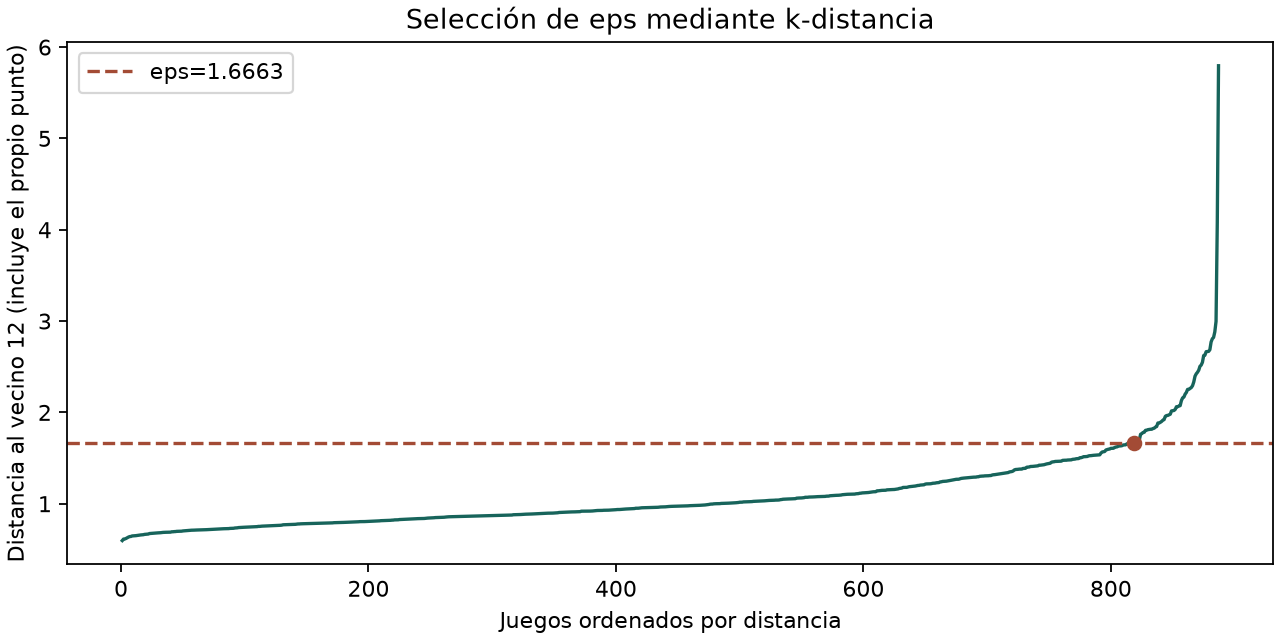
\includegraphics[width=\linewidth,height=.44\textheight,keepaspectratio]{figuras/clustering_03_dbscan_kdistancia.png}
\caption{Curva utilizada para seleccionar eps en Python.}\end{figure}\FloatBarrier

\section{Clasificación supervisada}\label{sec:clasificacion}
\subsection{Definición de popularidad relativa}
Comparamos conceptualmente dos objetivos. Solo Plays es más simple y representa alcance acumulado; el índice compuesto incorpora interés pendiente, aunque da dos tercios del peso a Wishlist y Backlogs, dos señales relacionadas. Se eligió el índice por ese alcance más amplio y se declara la redundancia como limitación:
\begin{equation}I(x)=\frac{P_{\mathrm{train}}(Plays_x)+P_{\mathrm{train}}(Wishlist_x)+P_{\mathrm{train}}(Backlogs_x)}{3}.\end{equation}
Los percentiles se ajustan como rangos medios divididos entre el tamaño del entrenamiento; para datos externos se interpolan entre valores distintos y se usan cero y uno fuera de sus extremos. Dos cortes en los terciles del índice de entrenamiento definen bajo, medio y alto, preservando empates. Estos niveles son relativos al catálogo popular, no umbrales absolutos de toda la industria.
\subsection{Separación y prevención de fuga}
Antes de definir etiquetas se aplica GroupShuffleSplit por título normalizado, semilla 42 y proporción aproximada 80/20: 892 registros de entrenamiento y 222 de prueba. No se exige estratificar clases que todavía no están definidas. La referencia del objetivo se calcula con entrenamiento y se aplica a ambos conjuntos.

La selección utiliza StratifiedGroupKFold de diez pliegues. Dentro de cada ajuste se recalculan referencia y cortes del objetivo, categorías e imputaciones usando solo el subentrenamiento. Las etiquetas de entrenamiento externo organizan los estratos, pero la puntuación de cada validación usa la referencia local. Esta distinción evita que la definición del objetivo conozca los conteos de la validación.

Las entradas del Pipeline son géneros, organizaciones, década y las dos notas. Ninguno de los cuatro conteos, el índice de popularidad, los clusters, PCA ni las banderas de procedencia entra al clasificador. El preprocesamiento forma parte del artefacto y recibe atributos crudos, tanto en las pruebas como en la web.
\subsection{Representación y comparación de modelos}
Los géneros se codifican multi-hot con hasta quince categorías y frecuencia mínima veinte dentro de cada ajuste. Las organizaciones usan frecuencia mínima diez; Otro se activa si no hay ninguna organización conocida. Las notas se imputan por mediana entrenada. La década se codifica mediante one-hot, conservando una categoría de ausencia.

La referencia es DummyClassifier con la clase más frecuente. CategoricalNB discretiza las notas en cinco intervalos; se prefiere a ajustar gaussianas sobre decenas de indicadores binarios raros, reconociendo la pérdida de resolución y la independencia aproximada. Se comparan además árbol CART y Random Forest. La selección se cierra por F1 macro media de CV antes de evaluar la prueba.

\begin{longtable}{p{0.174\textwidth}p{0.174\textwidth}p{0.174\textwidth}p{0.174\textwidth}p{0.174\textwidth}}
\caption{Comparación de producción. Exactitud expresada como fracción; prueba independiente de 222 casos.}\\
\toprule
Modelo & F1 CV & Desv CV & Exactitud prueba & F1 prueba\\\midrule\endfirsthead
Modelo & F1 CV & Desv CV & Exactitud prueba & F1 prueba\\\midrule\endhead
Dummy & 0.1678 & 0.0031 & 0.3018 & 0.1546\\
Naive Bayes & 0.5490 & 0.0625 & 0.5090 & 0.4925\\
Árbol CART & 0.5053 & 0.0458 & 0.5315 & 0.5119\\
Random Forest & 0.5567 & 0.0451 & 0.5676 & 0.5577\\
\bottomrule\end{longtable}

Random Forest obtiene el mejor F1 de CV, 0.5567. Sus 200 árboles usan semilla 42, profundidad sin límite y mínimo de cinco ejemplos por hoja. En prueba logra F1 macro 0.5577 y exactitud 56.76\,\%, frente a F1 0.1546 de Dummy. La diferencia es amplia dentro de esta partición, pero no se realizó una prueba de significancia ni validación externa.

La matriz, en orden bajo, medio y alto para filas reales y columnas predichas, es:
\begin{equation}\begin{pmatrix}43&14&10\\32&27&21\\9&10&56\end{pmatrix}.\end{equation}
Al revisar la matriz se observa que la clase media es el problema más claro del modelo: de ochenta juegos que realmente pertenecían a ese nivel, solamente veintisiete fueron identificados correctamente. Los demás se repartieron entre bajo y alto. Esto nos muestra que no era suficiente presentar únicamente la exactitud general, porque esa cifra podía ocultar una dificultad importante. Una explicación posible es que los juegos cercanos a las fronteras de los terciles compartan atributos con ambos extremos, aunque este experimento no permite demostrar que esa sea la causa.
\subsection{Interpretación y revisión del entrenamiento}
La importancia por permutación mide la caída de F1 macro al permutar entradas crudas en prueba, con treinta repeticiones y semilla 42. Rating y Metacritic aportan las mayores caídas medias. No es una atribución causal; las variables correlacionadas pueden compartir información. Las barras muestran desviación de repeticiones, no intervalos de confianza inferenciales.

\begin{figure}[htbp]\centering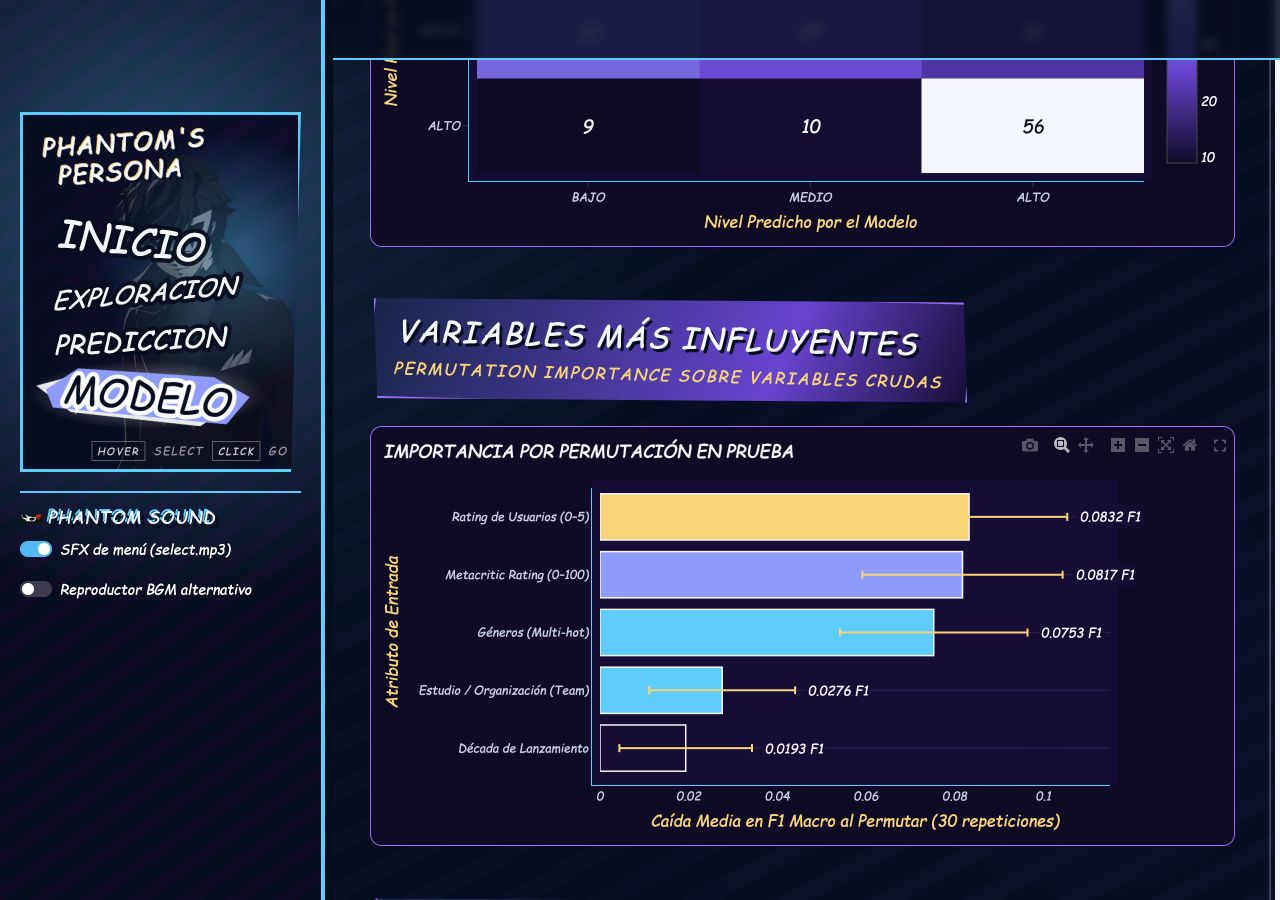
\includegraphics[width=\linewidth,height=.51\textheight,keepaspectratio]{figuras/graficas_permutacion_corregida.jpg}
\caption{Importancia por permutación mostrada en la web. Las cifras se separan del extremo de las barras de error.}\end{figure}\FloatBarrier

\begin{longtable}{p{0.29\textwidth}p{0.29\textwidth}p{0.29\textwidth}}
\caption{Auditoría adicional con el vigente y siete variantes del bosque, usando únicamente entrenamiento.}\\
\toprule
Candidato & F1 CV & Recall medio CV\\\midrule\endfirsthead
Candidato & F1 CV & Recall medio CV\\\midrule\endhead
Vigente & 0.5567 & 0.3385\\
RF\_\allowbreak{}revision\_\allowbreak{}3 & 0.5510 & 0.3289\\
RF\_\allowbreak{}revision\_\allowbreak{}2 & 0.5508 & 0.3592\\
RF\_\allowbreak{}revision\_\allowbreak{}4 & 0.5427 & 0.2942\\
RF\_\allowbreak{}revision\_\allowbreak{}1 & 0.5403 & 0.3796\\
RF\_\allowbreak{}revision\_\allowbreak{}5 & 0.5374 & 0.3794\\
RF\_\allowbreak{}revision\_\allowbreak{}7 & 0.5368 & 0.3491\\
RF\_\allowbreak{}revision\_\allowbreak{}6 & 0.5300 & 0.3623\\
\bottomrule\end{longtable}

Se hicieron ochenta ajustes, ocho candidatos por diez pliegues, variando mínimo por hoja, ponderación y número de variables por división. El criterio previo de sustitución exigía al menos 0.01 de mejora en F1 macro y superioridad en seis pliegues. Ninguna variante superó la media del modelo vigente y no se reemplazó el artefacto.

La búsqueda amplía la exploración sobre los mismos pliegues y no es una CV anidada. La prueba histórica ya fue observada. Por ello no afirmamos que estas medias midan mejora prospectiva ni presentamos un entrenamiento nuevo como mejor solo por haberlo ejecutado.
\section{Corridas gráficas y contraste con Weka}\label{sec:weka}
Weka Explorer 3.8.7 es la herramienta de la materia utilizada para contrastar clasificación y clustering \parencite{frank2016weka,wekaweb}. Se conservaron las salidas completas y capturas de seis corridas. No se atribuyen a Orange los resultados de Weka.

La clasificación usa 892 instancias y 53 atributos, incluida nivel\_popularidad nominal, con diez pliegues. Las cuatro matrices se recalcularon: cada una suma 892 y sus diagonales reproducen la exactitud mostrada por el programa. El F1 macro se obtiene del promedio simple de F Measure por clase impreso; el ponderado se toma de Weighted Avg salvo ZeroR, donde los valores no definidos se resuelven desde la matriz y se identifican como calculados.

\begin{table}[htbp]\centering\caption{Clasificación en Weka sobre 892 casos.}\begin{tabular}{lrrr}\toprule Modelo&Exactitud (\%)&F1 macro&F1 ponderado\\\midrule
ZeroR & 33.0717 & 0.2533 & 0.2533\\
NaiveBayes & 50.8969 & 0.5033 & 0.5030\\
J48 & 51.0090 & 0.5063 & 0.5060\\
RandomForest & 53.4753 & 0.5300 & 0.5300\\
\bottomrule\end{tabular}\end{table}
\begin{figure}[htbp]\centering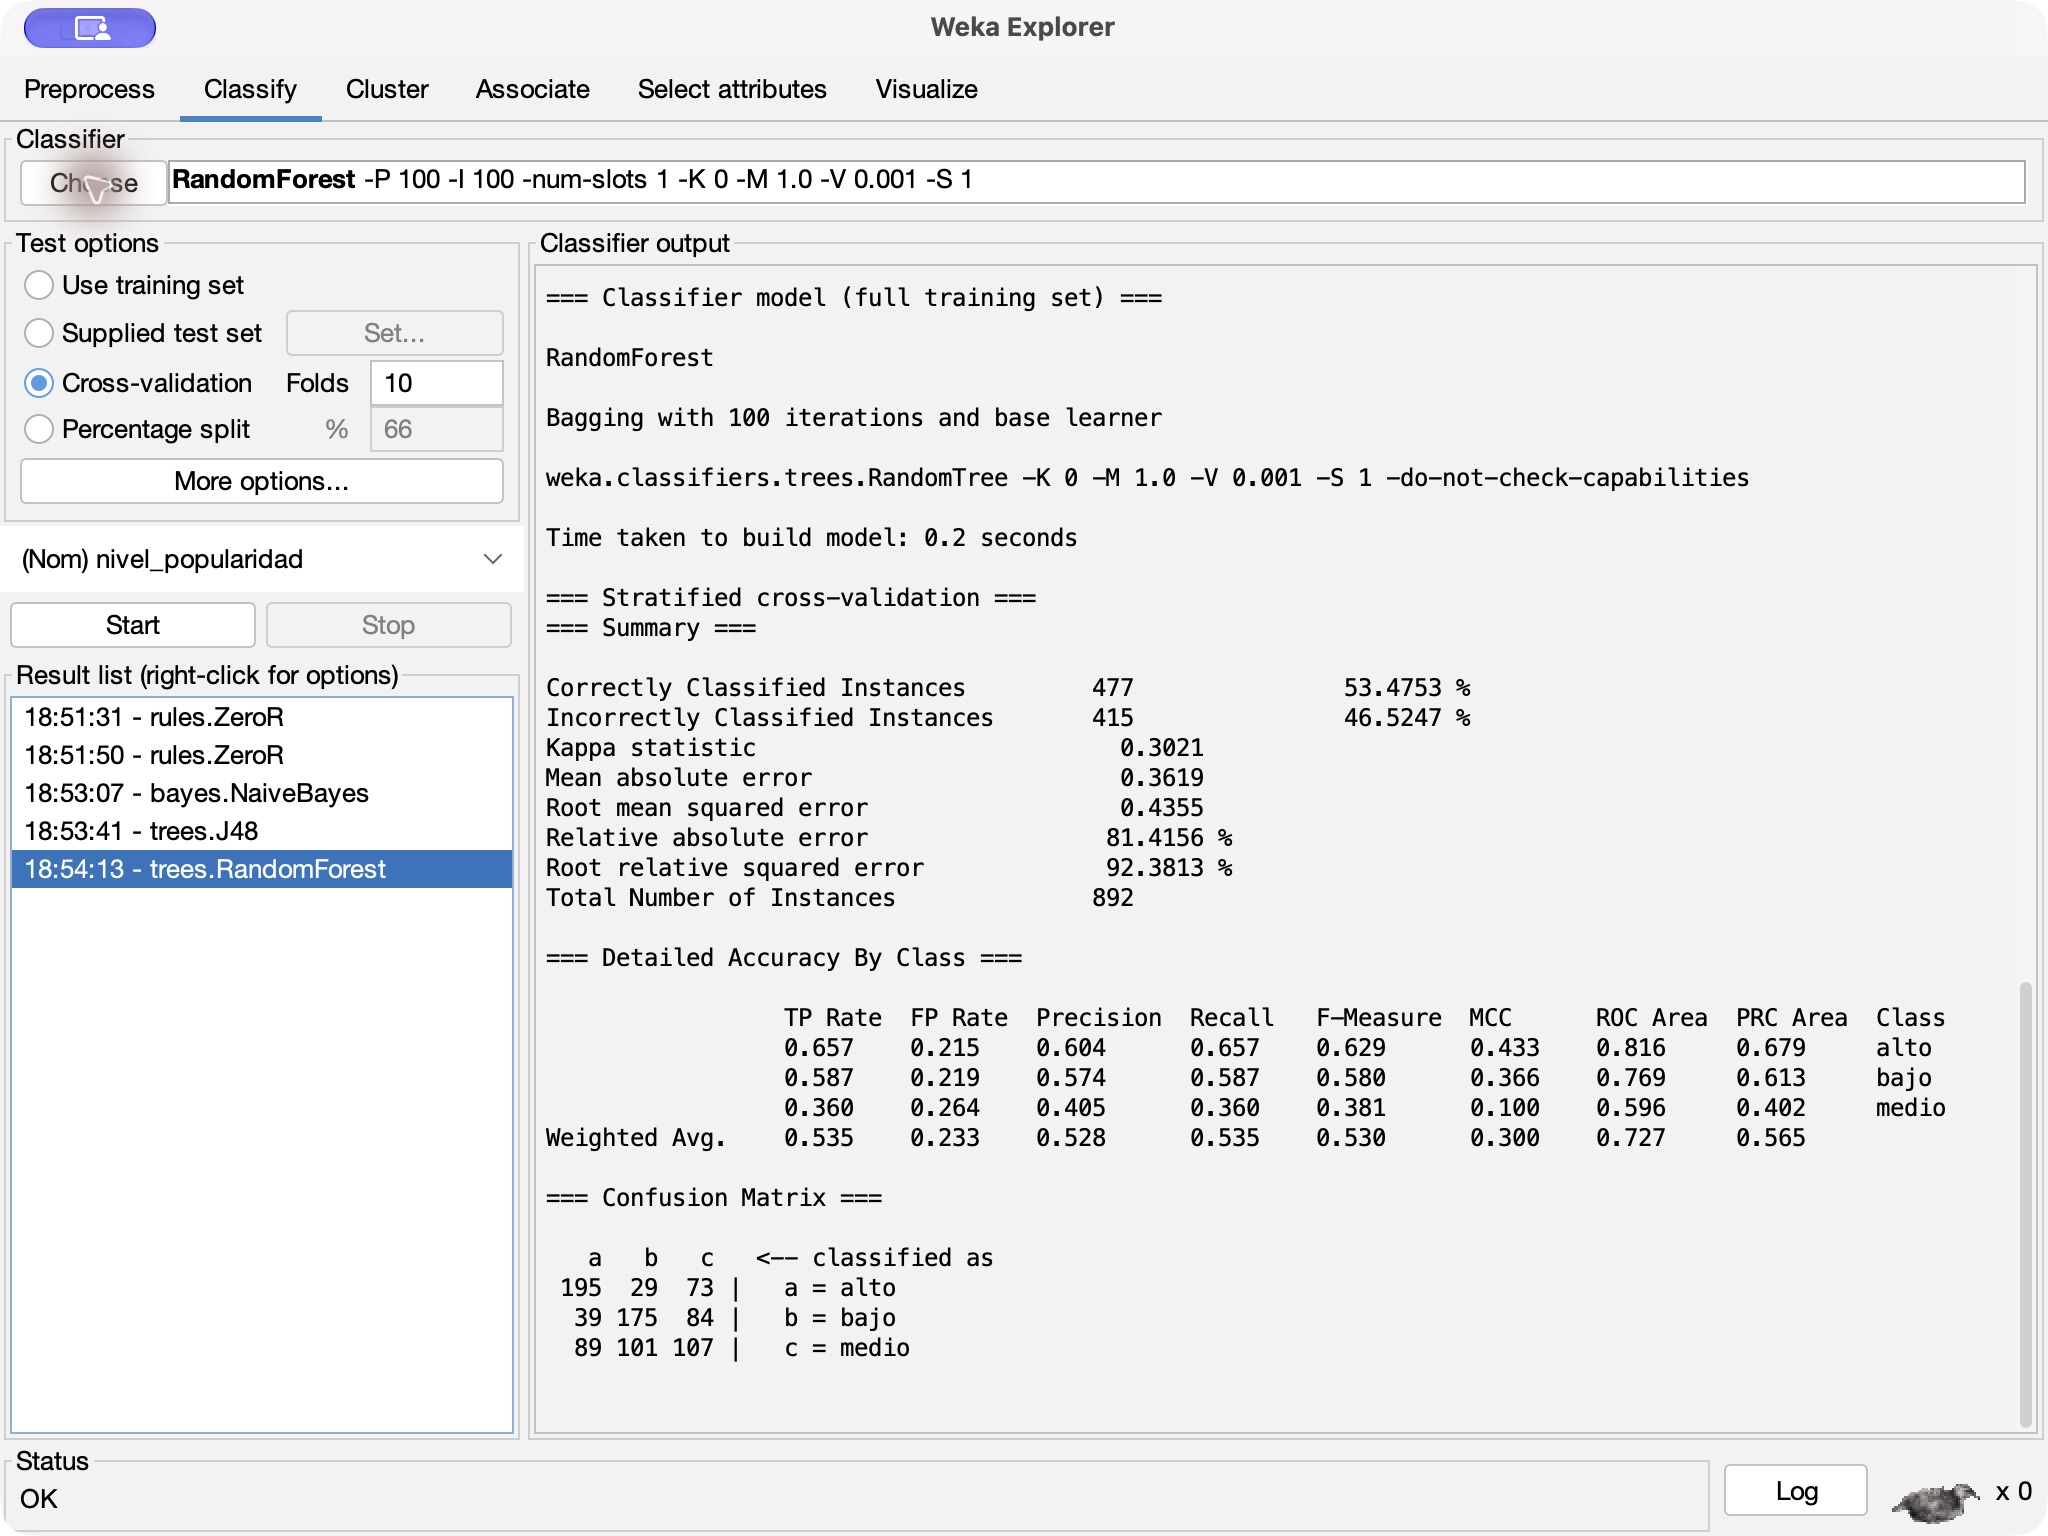
\includegraphics[width=\linewidth,height=.6\textheight,keepaspectratio]{figuras/RandomForest.png}
\caption{Evidencia de la corrida gráfica de RandomForest en Weka; incluye resumen, métricas por clase y matriz.}\end{figure}\FloatBarrier

RandomForest fue el mejor de las cuatro corridas, con 477 aciertos. Su recall de medio fue 0.360, lo que coincide cualitativamente con la dificultad de la clase central en Python. Sin embargo, no se debe comparar directamente su 53.4753\,\% con el 56.76\,\% de prueba de la app: son poblaciones y protocolos distintos.

La comparación de enlace de Python usa los mismos 892 registros y 52 atributos numéricos exportados. Allí Random Forest obtiene 54.8206\,\% y F1 macro 0.5442. Las particiones Java y sklearn no son idénticas, la semilla de CV de la sesión Weka no se recuperó, y los algoritmos difieren: J48 no es CART; Weka NaiveBayes no garantiza estimadores numéricos iguales a GaussianNB. Weka RandomForest usa cien árboles y semilla del estimador uno, frente a cien y 42 en el enlace de Python.

Además, el preprocesamiento de los archivos exportados ocurre antes de la CV de enlace. Ese contraste sirve para comparación descriptiva entre herramientas, pero no sustituye el protocolo de producción con categorías e imputaciones locales por pliegue. El archivo comparativo conserva también evaluaciones de Python sobre 1,117 y 1,114 casos, identificando cada universo.

En SimpleKMeans se usaron dos grupos y semilla 42. Se obtuvieron 477 y 410 casos tras nueve iteraciones; en Python fueron 465 y 422. Los centros de Weka son positivos en las seis variables para el primer grupo y negativos para el segundo, compatibles con una separación por magnitud conjunta. La suma de cuadrados de Weka, 76.6310, no se compara con la de Python como si ambas configuraciones de distancia fueran idénticas.

\begin{figure}[htbp]\centering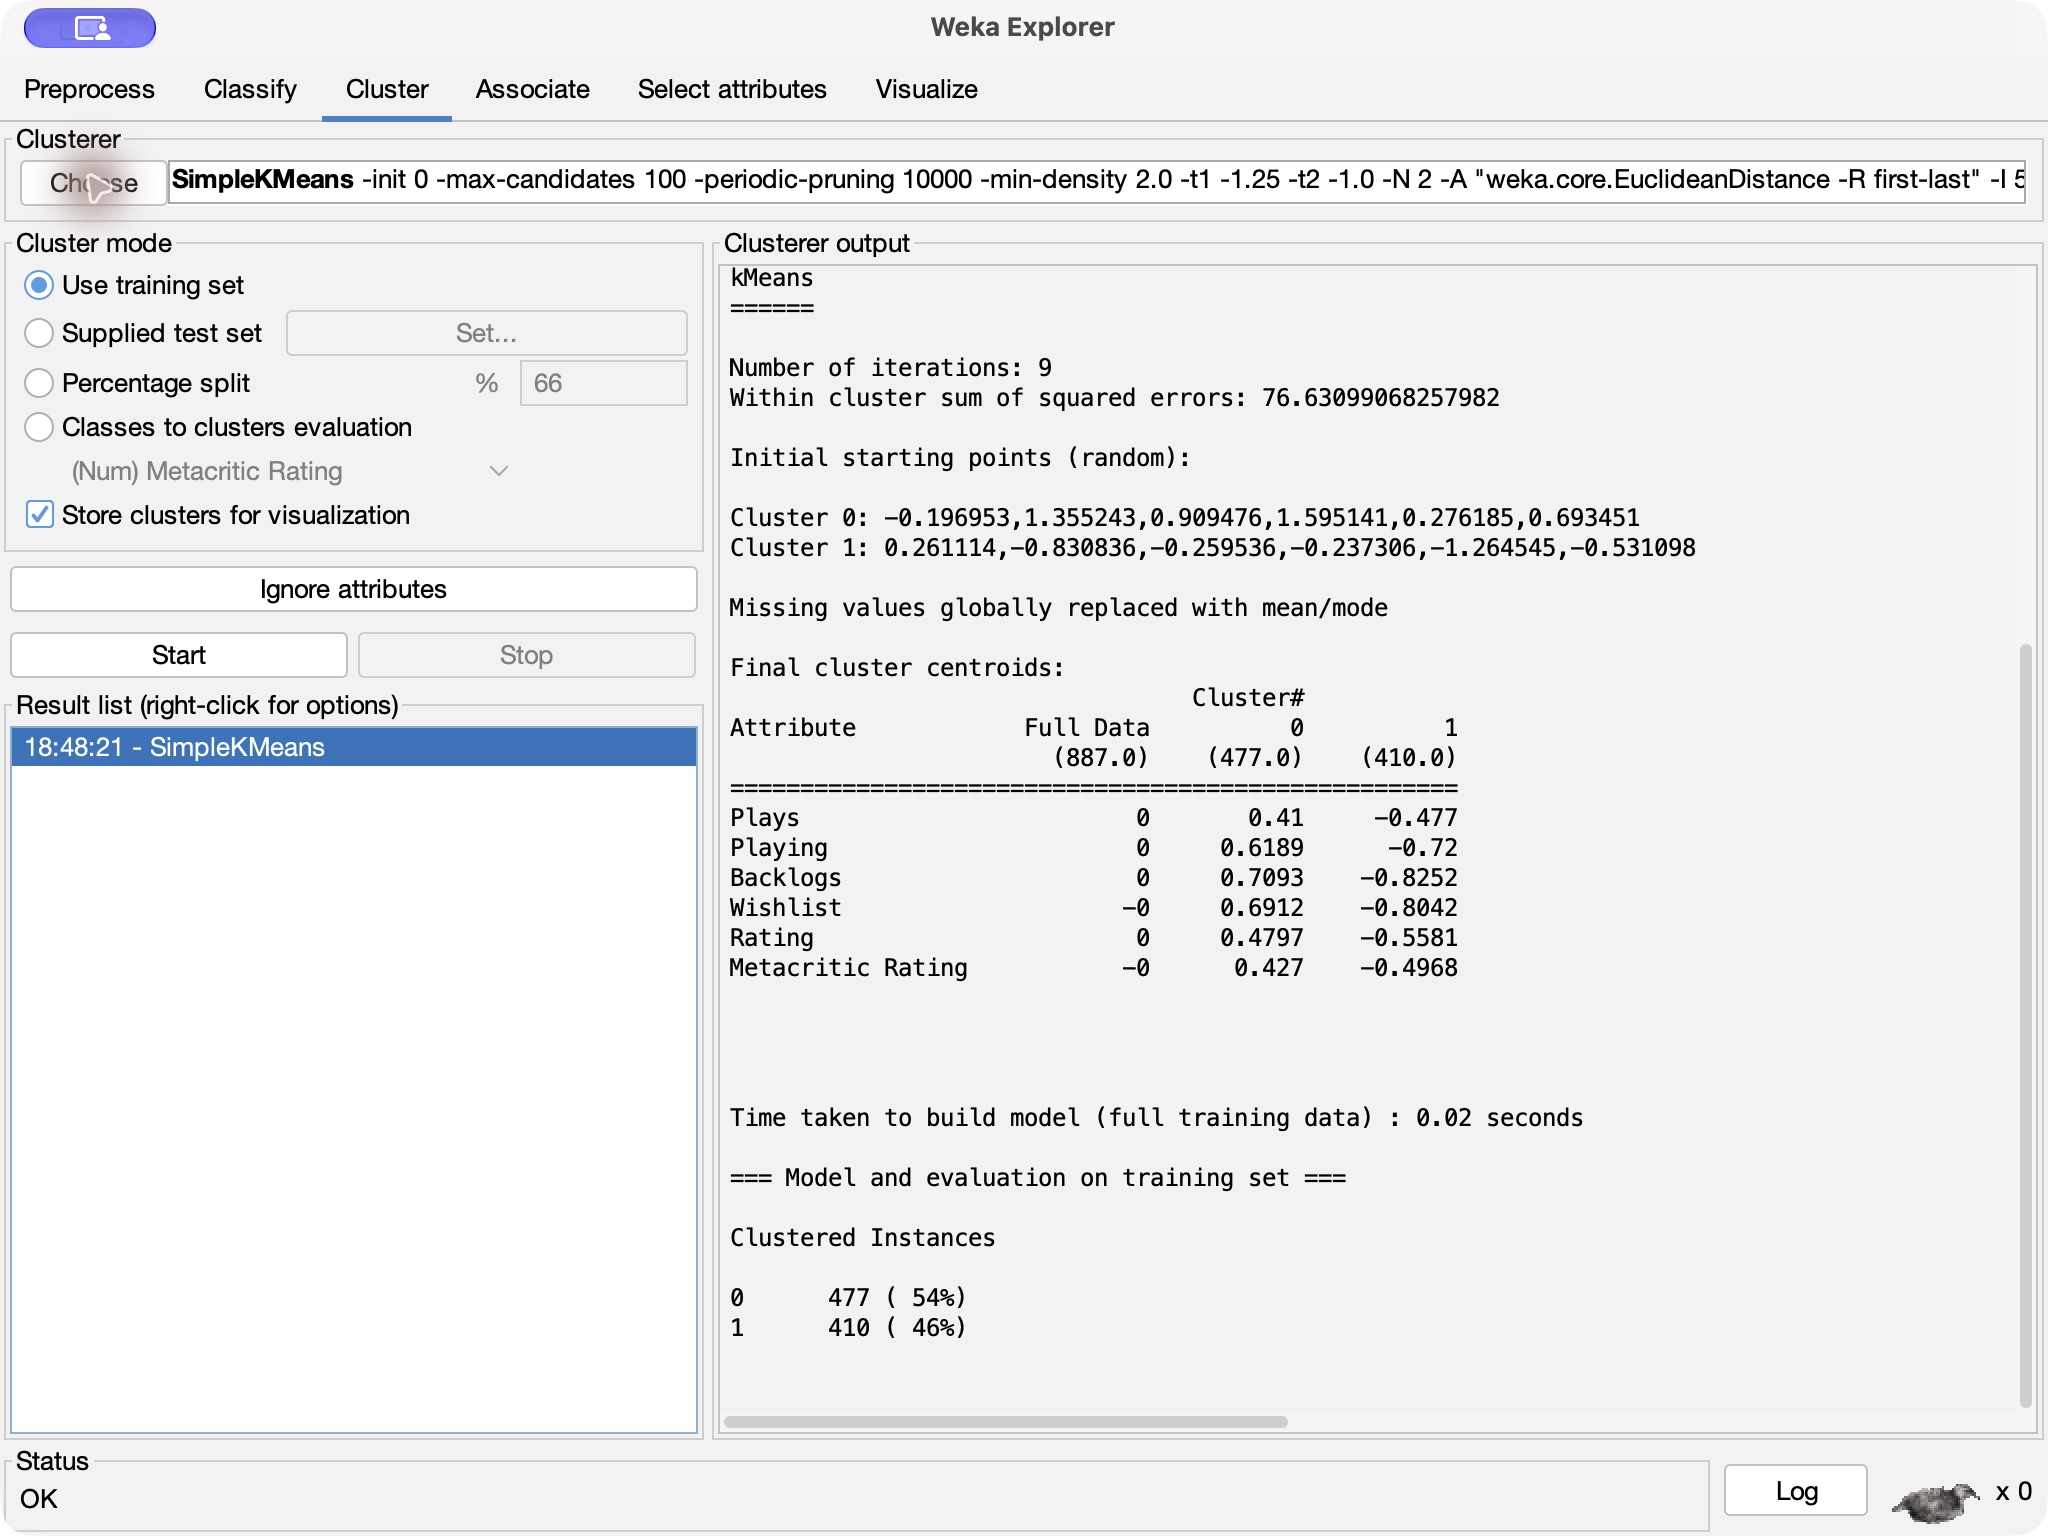
\includegraphics[width=\linewidth,height=.55\textheight,keepaspectratio]{figuras/kmeans_resultado.png}
\caption{Salida gráfica de SimpleKMeans en Weka. Los centroides corresponden a las variables exportadas transformadas.}\end{figure}\FloatBarrier

Weka DBSCAN, con eps 1.666296 y minPoints doce, agrupó los 887 casos en un solo grupo sin ruido. Python dejó veintiún puntos como ruido. Compartir parámetros nominales no demuestra equivalencia de la distancia interna de EuclideanDistance y la implementación de sklearn. No se modificaron resultados ni se ajustó eps para forzar coincidencia.

\begin{figure}[htbp]\centering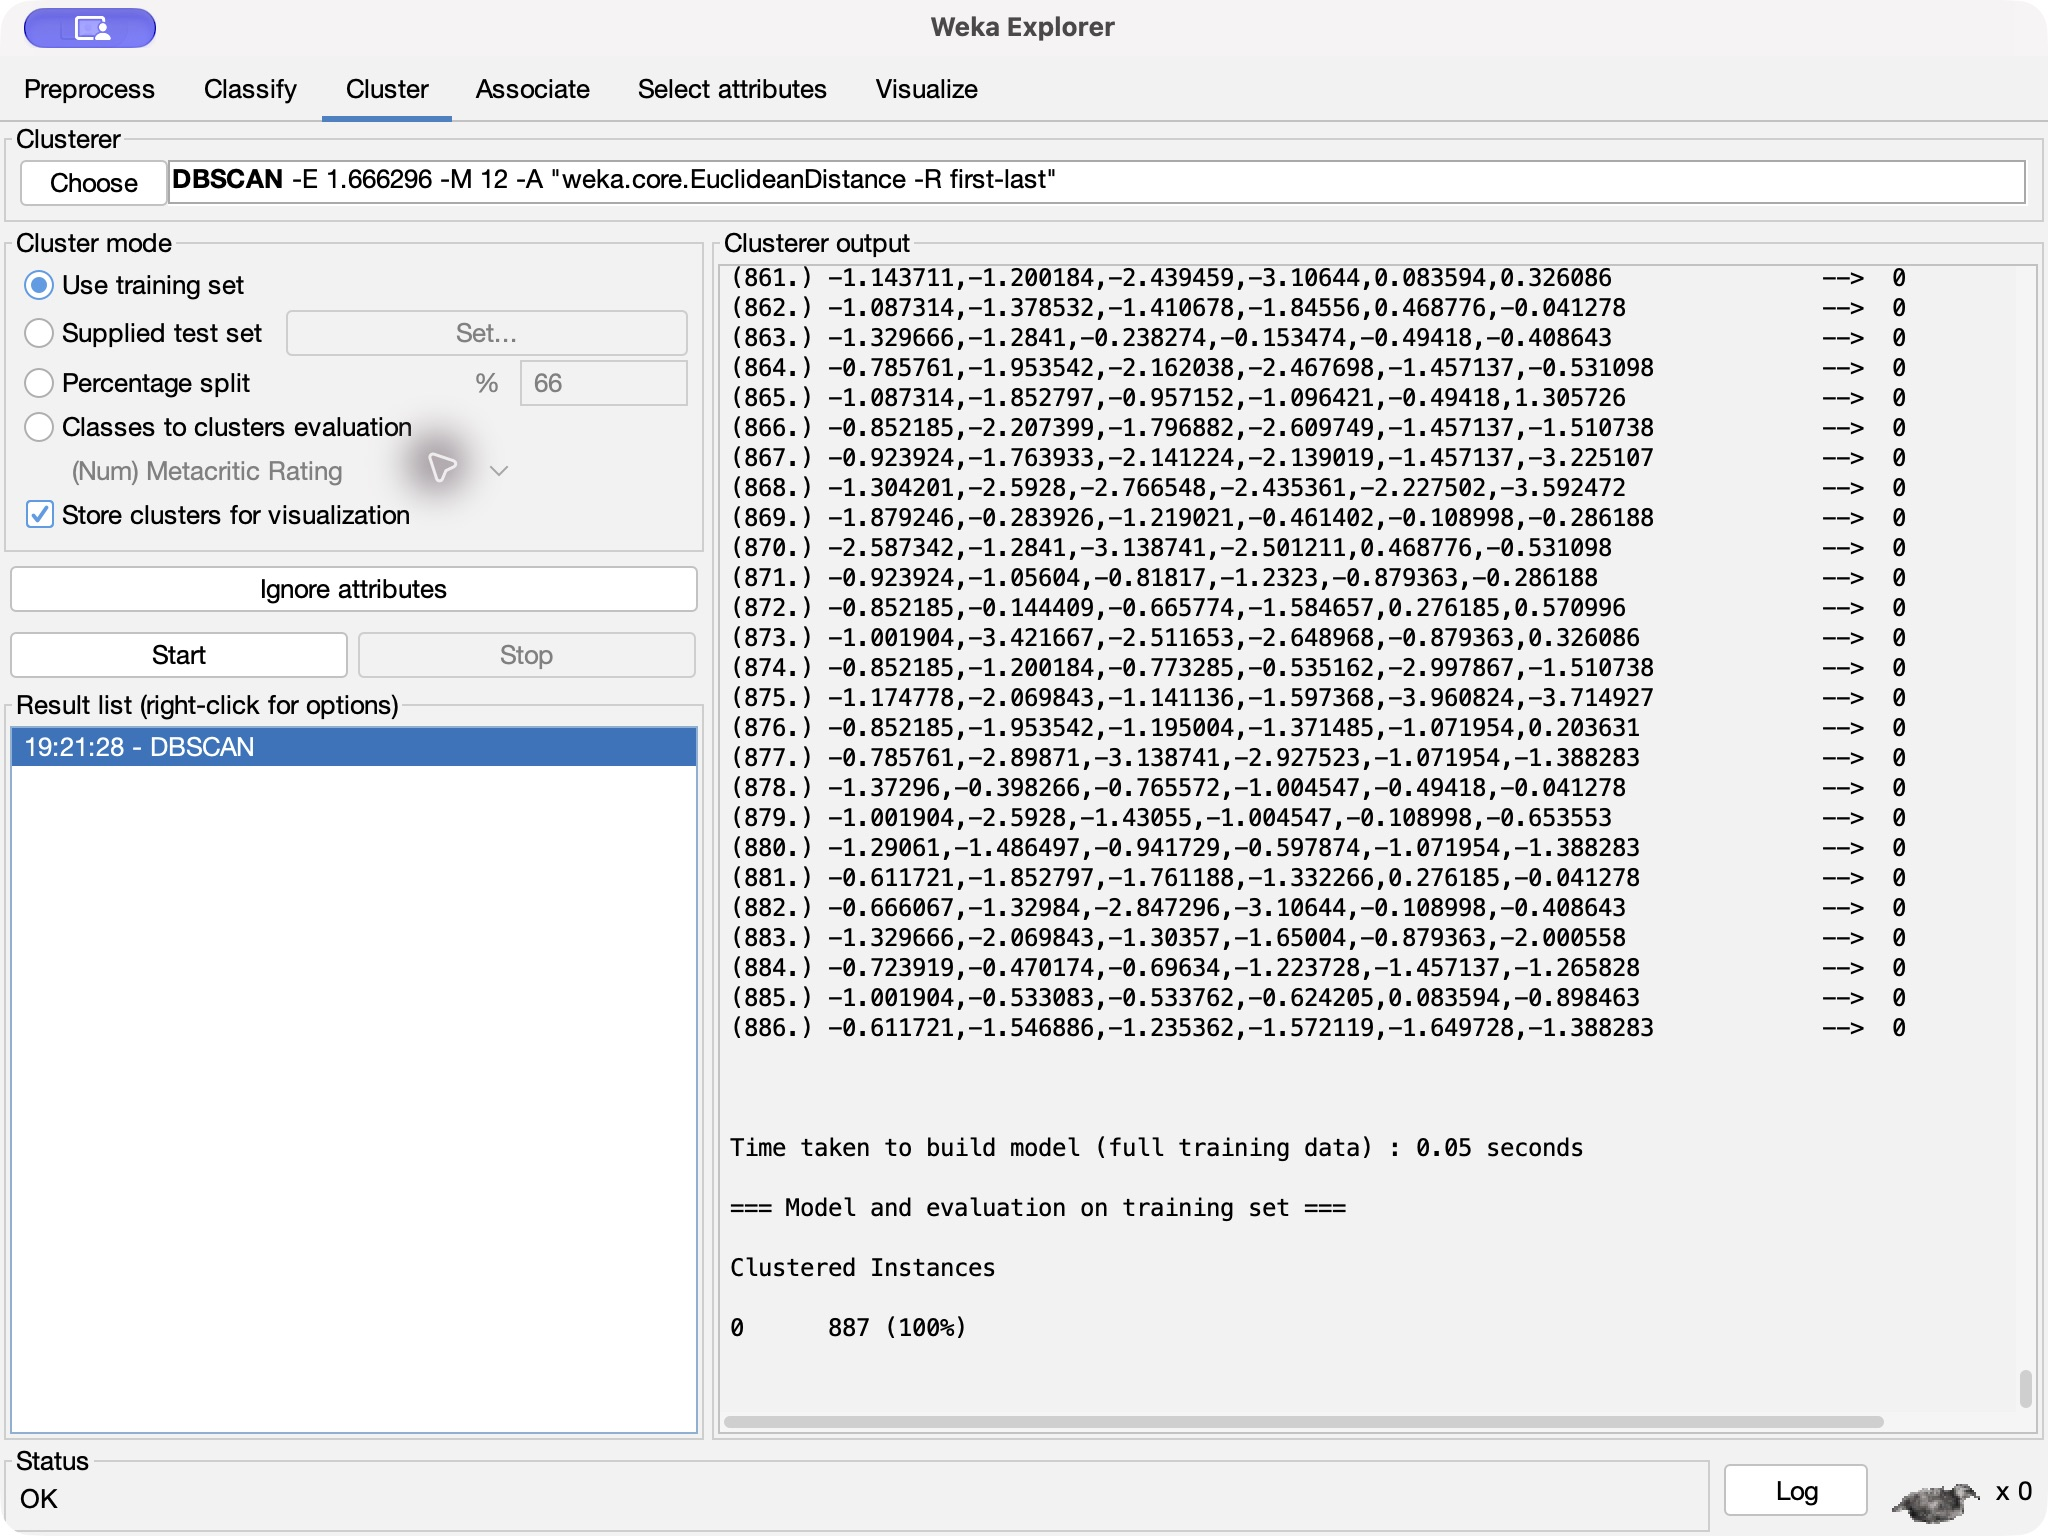
\includegraphics[width=\linewidth,height=.52\textheight,keepaspectratio]{figuras/dbscan_resultado.png}
\caption{Salida original de DBSCAN en Weka. Un grupo dominante no demuestra múltiples segmentos de mercado.}\end{figure}\FloatBarrier

Orange no produjo evaluaciones utilizables. Hubo cierres en Qt/Cocoa al emplear selectores; se probaron instalación local, recuperación y reinicio del lienzo, importación CSV y TAB y un lanzador con selectores Qt. El cierre de esta vía se documentó como desviación del plan. Power BI no se utilizó y no hay una corrida MLP que pueda reportarse.
\section{Aplicación y demostración}\label{sec:web}
La web se implementó en Streamlit con cuatro páginas. Inicio presenta alcance, límites y consulta del catálogo. Exploración ofrece señales, brechas y perfiles; Predicción recibe atributos crudos y muestra la clase y sus probabilidades; Modelo documenta resultados por algoritmo, errores por clase y el diagnóstico de ausencias. El artefacto incluye su preprocesamiento y los vecinos se calculan exclusivamente en el espacio predictivo de entrenamiento.

El formulario utiliza géneros, organización, década y notas. No solicita Plays ni listas de interés porque serían las señales con las que se construyó la respuesta. Las pruebas comparan sus salidas con el Pipeline y usan el orden real de clases; una inversión entre el orden de las probabilidades y el de las etiquetas habría producido una interfaz errónea aun con un buen modelo.

\begin{figure}[htbp]\centering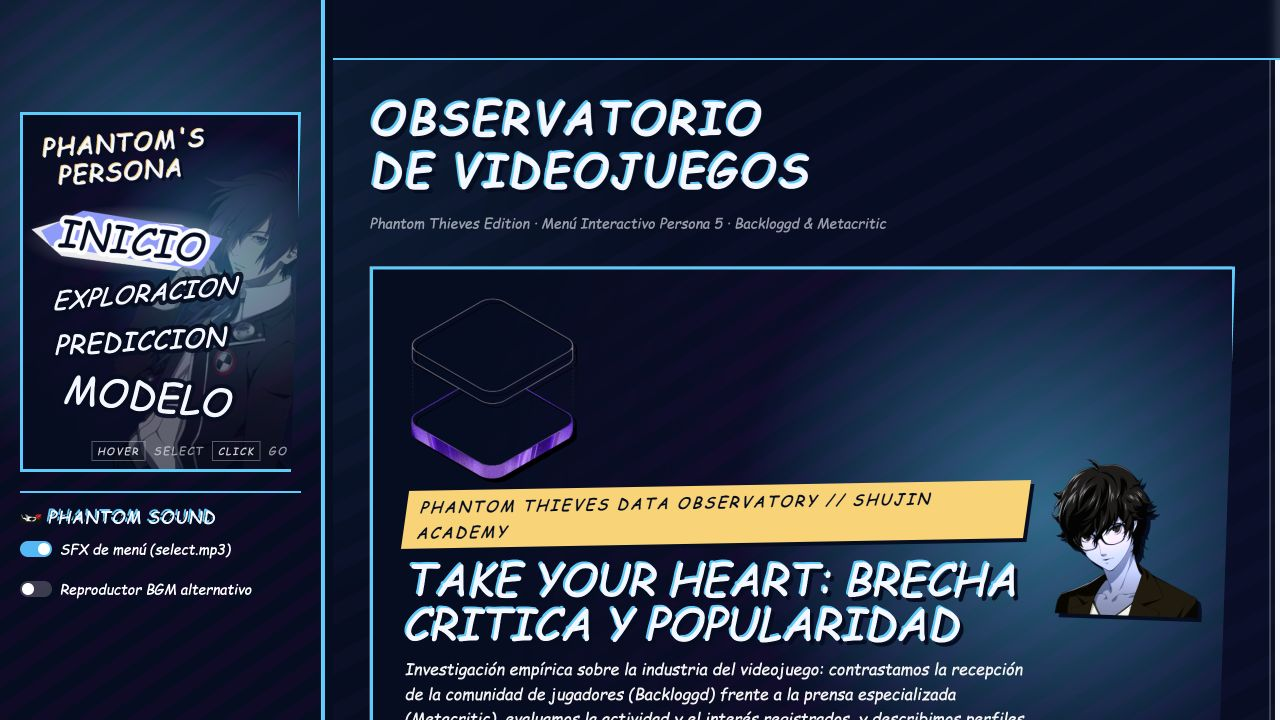
\includegraphics[width=\linewidth,height=.44\textheight,keepaspectratio]{figuras/inicio_actual.jpg}
\caption{Página Inicio capturada durante la integración del documento, el 9 de noviembre de 2026.}\end{figure}\FloatBarrier

\begin{figure}[htbp]\centering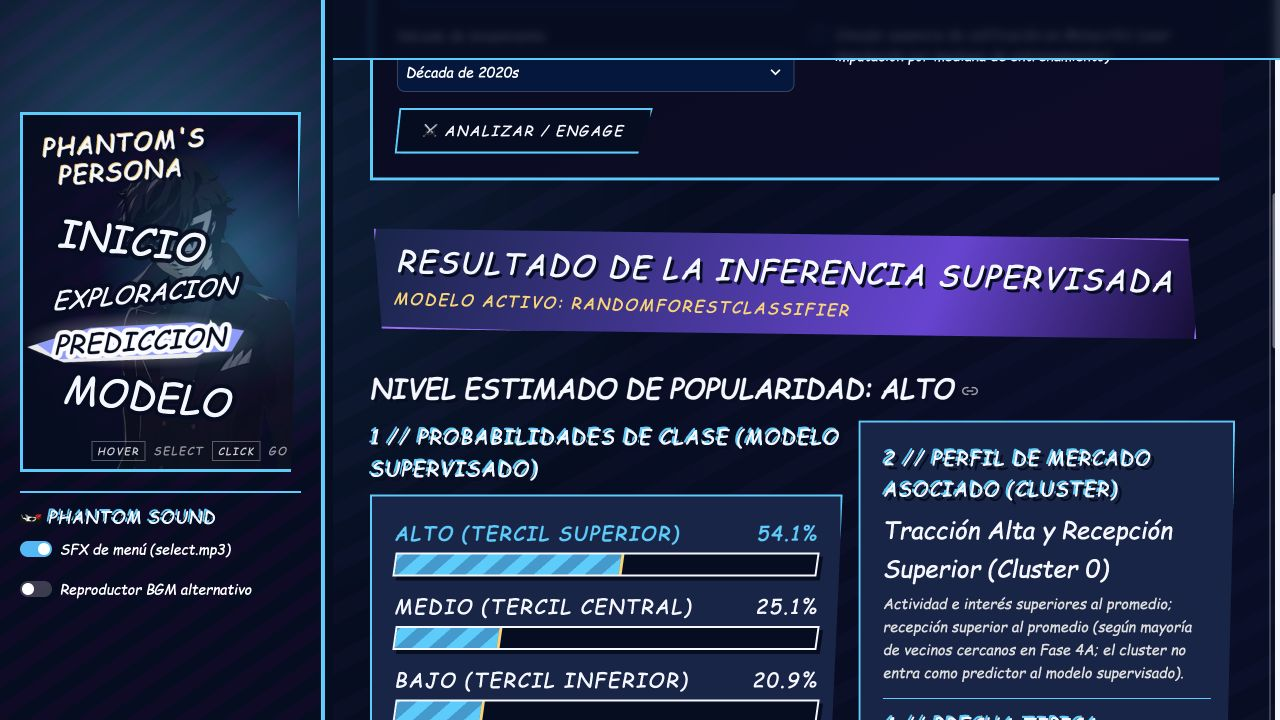
\includegraphics[width=\linewidth,height=.5\textheight,keepaspectratio]{figuras/formulario_verificado.jpg}
\caption{Demostración verificada: Adventure y RPG, Otro, década 2020, Rating 5 y Metacritic 100 producen alto con 54.1 por ciento no calibrado.}\end{figure}\FloatBarrier

En ese caso, ocultar Metacritic manteniendo Rating cinco cambia la clase a bajo con 44.2\,\%. El cálculo coincide con el modelo guardado; no es un error de etiqueta del formulario. Se añadió un aviso visible de imputación porque la ausencia de prensa no implica mala recepción. Esta sensibilidad muestra el límite de usar cobertura de prensa en un catálogo curado, incluso sin una bandera explícita de ausencia como predictor.

\begin{figure}[htbp]\centering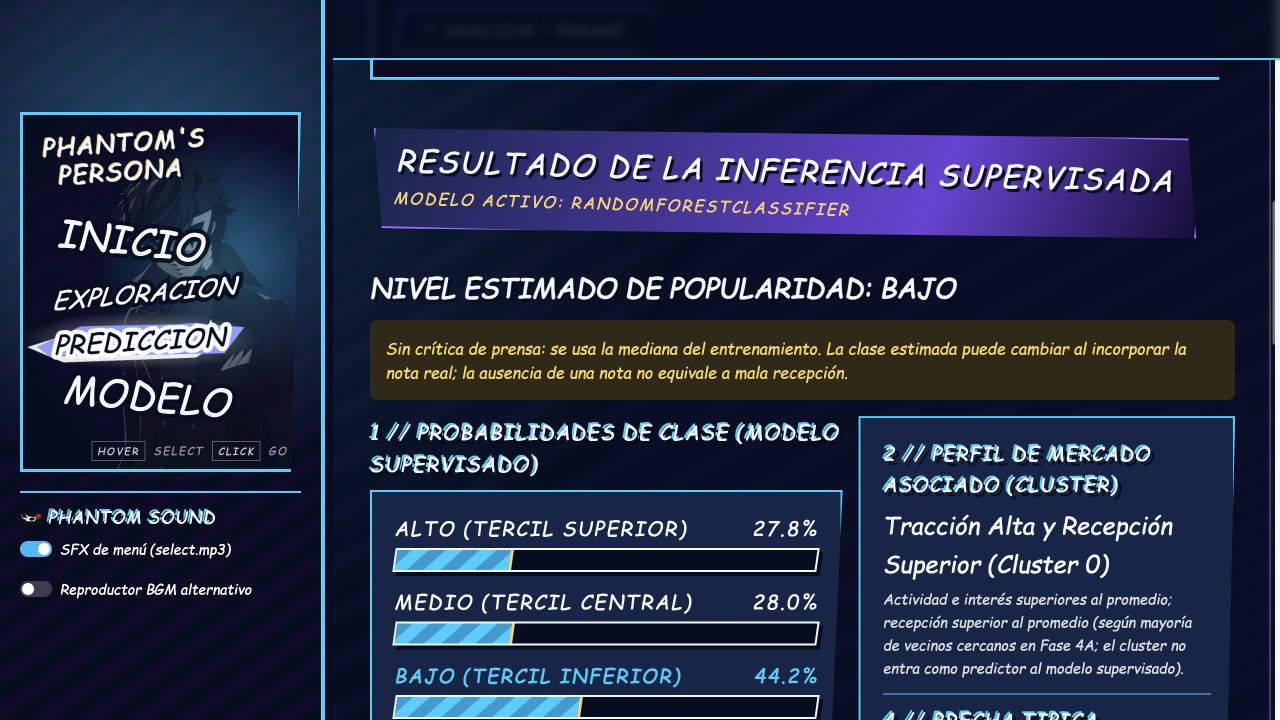
\includegraphics[width=\linewidth,height=.48\textheight,keepaspectratio]{figuras/sin_critica_verificado.jpg}
\caption{Aviso y resultado del caso sin calificación crítica. El cambio no se interpreta como certeza de baja popularidad.}\end{figure}\FloatBarrier

La identidad gráfica combina azul marino, morado, cian y dorado con fuente cómic local. Se centralizaron colores, se separaron etiquetas de barras de error, se quitaron marcas logarítmicas menores amontonadas y se dio ancho suficiente a las figuras. En móvil, las gráficas densas conservan lectura mediante desplazamiento horizontal dentro del panel. Estos cambios son de presentación: no alteran escalas estadísticas ni mediciones.

Se corrigió también el mínimo visual artificial de dos por ciento en las barras de probabilidad y la etiqueta que confundía una organización no frecuente con un estudio independiente. Los inputs validan escalas y dejan los nulos a la imputación entrenada. Las probabilidades no están calibradas y no se presentan como posibilidades actuariales de éxito.

La aplicación se entrega para ejecución local con \texttt{streamlit run app.py} desde Final. No se desplegó en Community Cloud ni se subió el dataset a GitHub por instrucción del usuario. La demo local satisface la comprobación funcional, pero no equivale a una publicación accesible públicamente.
\section{Escenarios de predicción y contrastación del modelo}\label{sec:escenarios}
\subsection{Qué queríamos comprobar con los escenarios}
Después de revisar la exactitud general, todavía quedaba una pregunta importante: ¿cómo se comporta el modelo cuando cambiamos las características de un videojuego? Para responderla planteamos situaciones concretas y mantuvimos fijas las demás entradas. La intención no fue buscar ejemplos que hicieran ver bien al modelo, sino mostrar qué información parece pesar en sus respuestas y en qué situaciones conviene cuestionarlas.

Se separaron dos tipos de prueba. Los escenarios hipotéticos permiten revisar sensibilidad, pero no tienen una clase real observada; por eso no pueden demostrar por sí solos que una respuesta sea correcta o incorrecta. Para refutar predicciones concretas también recuperamos juegos del conjunto de prueba y comparamos la clase estimada con la clase calculada a partir de sus señales de popularidad. Estos ejemplos ya forman parte de la evaluación histórica: no constituyen una muestra nueva ni una nueva medición del rendimiento.
\subsection{Escenarios con cambios controlados}
El escenario de referencia utiliza Adventure y RPG, organización Otro y década de 2020. En S1 a S5 únicamente se modifican las calificaciones y la presencia de prensa. S6 cambia la organización a Nintendo; S7 cambia la década a 1980; S8 utiliza Shooter. Se trata de comparaciones de entradas del mismo modelo, no de afirmaciones causales sobre esas organizaciones o géneros.
\begin{longtable}{p{.08\textwidth}p{.28\textwidth}p{.11\textwidth}p{.11\textwidth}p{.12\textwidth}p{.14\textwidth}}
\caption{Escenarios hipotéticos calculados con el Pipeline guardado. La última columna muestra la mayor probabilidad, sin calibrar.}\\\hline
Caso&Situación&Rating&Prensa&Predicción&Probabilidad\\\hline\endfirsthead
Caso&Situación&Rating&Prensa&Predicción&Probabilidad\\\hline\endhead
S1 & Notas bajas & 1.0 & 45 & bajo & 60.0\%\\\hline
S2 & Notas altas & 4.8 & 99 & alto & 54.1\%\\\hline
S3 & Usuarios altos y prensa baja & 4.8 & 45 & bajo & 43.9\%\\\hline
S4 & Usuarios bajos y prensa alta & 1.0 & 99 & alto & 38.2\%\\\hline
S5 & Usuarios altos sin prensa & 4.8 & Ausente & bajo & 44.2\%\\\hline
S6 & Cambio de organización & 4.8 & 99 & alto & 58.7\%\\\hline
S7 & Cambio de década & 4.8 & 99 & alto & 57.2\%\\\hline
S8 & Cambio de género & 4.8 & 99 & alto & 49.7\%\\\hline
\end{longtable}
Al comparar S1 y S2 se observa el comportamiento que esperaríamos en una primera revisión: con ambas notas bajas se estima bajo y con ambas altas se estima alto. Sin embargo, los casos cruzados muestran una situación menos sencilla. S3 tiene Rating de 4.8 y prensa de 45, pero el modelo responde bajo con 43.9\,\%. En S4 sucede lo contrario: Rating de 1.0 y prensa de 99 producen alto con solamente 38.2\,\%. Es la clase con mayor probabilidad, pero ni siquiera alcanza la mitad. Esto impide presentar esa etiqueta como una respuesta segura.

S5 conserva la calificación de usuarios de S2 y oculta Metacritic. La predicción cambia de alto a bajo, con 44.2\,\% para bajo. Esta comparación cuestiona una lectura demasiado simple de la pantalla: que falte una nota no significa que la prensa haya evaluado mal al juego. El resultado aparece porque el Pipeline sustituye el dato ausente por su mediana entrenada y el bosque utiliza esa entrada junto con las demás variables. La web conserva un aviso para que esa situación no pase desapercibida.

También se observa que cambiar únicamente la organización o la década modifica las probabilidades, aunque en estos ejemplos se mantiene la clase alta. No podemos concluir que Nintendo o una década causen popularidad; solo estamos describiendo cómo responde un modelo entrenado sobre este catálogo. En S8, cambiar los géneros por Shooter deja alto como primera clase con 49.7\,\%, otra respuesta que debe leerse con cautela.
\begin{figure}[htbp]\centering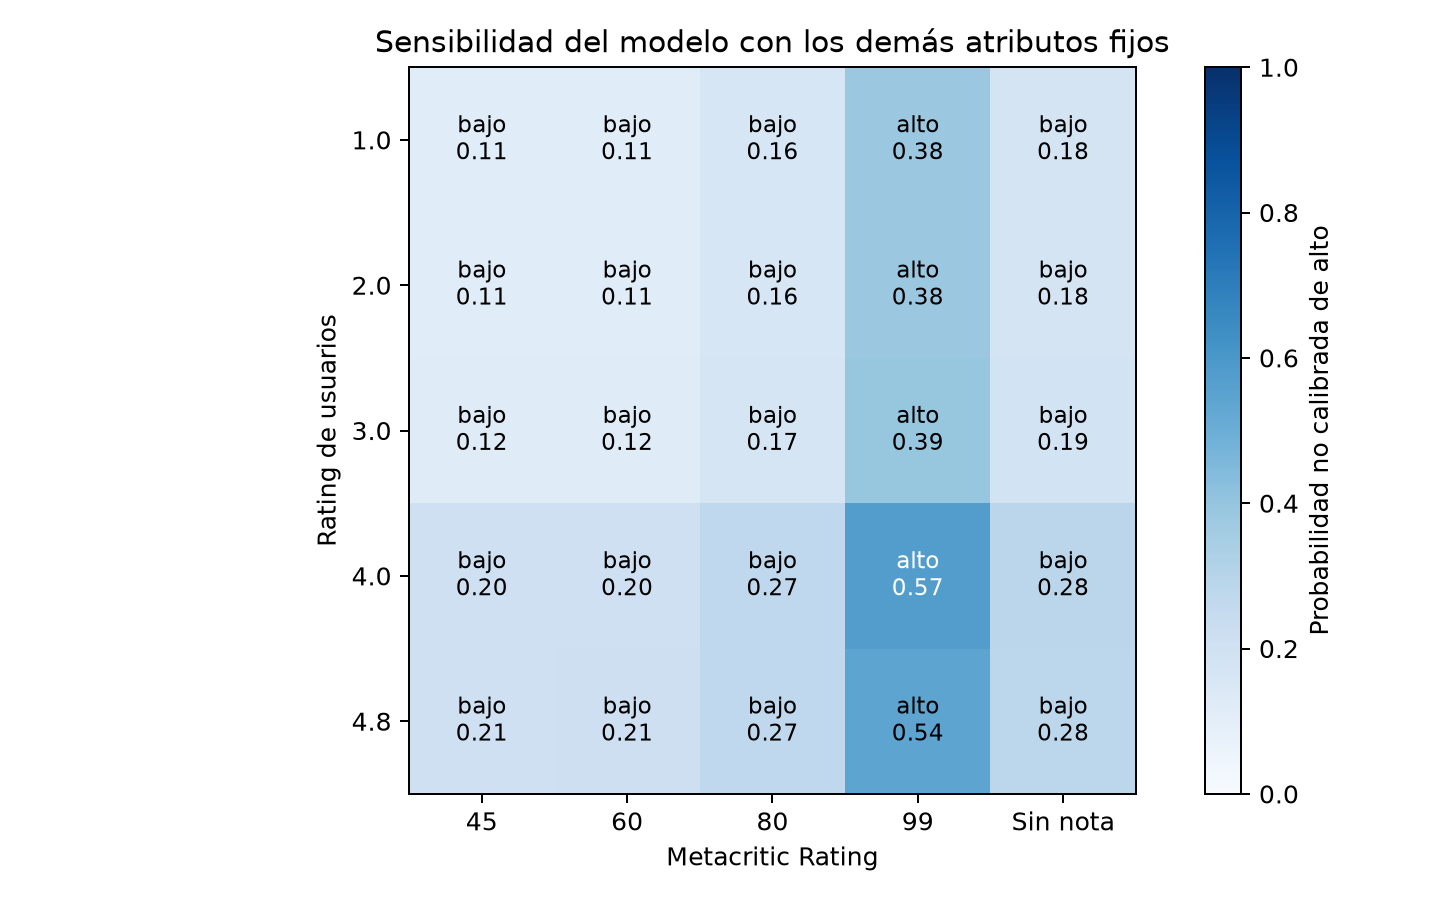
\includegraphics[width=\linewidth]{figuras/sensibilidad_escenarios.png}\caption{Veinticinco combinaciones de Rating y Metacritic con el resto de atributos fijos. La etiqueta es la clase estimada y el color muestra la probabilidad no calibrada de alto.}\end{figure}\FloatBarrier
\subsection{Resultados capturados en el formulario}
\begin{figure}[htbp]\centering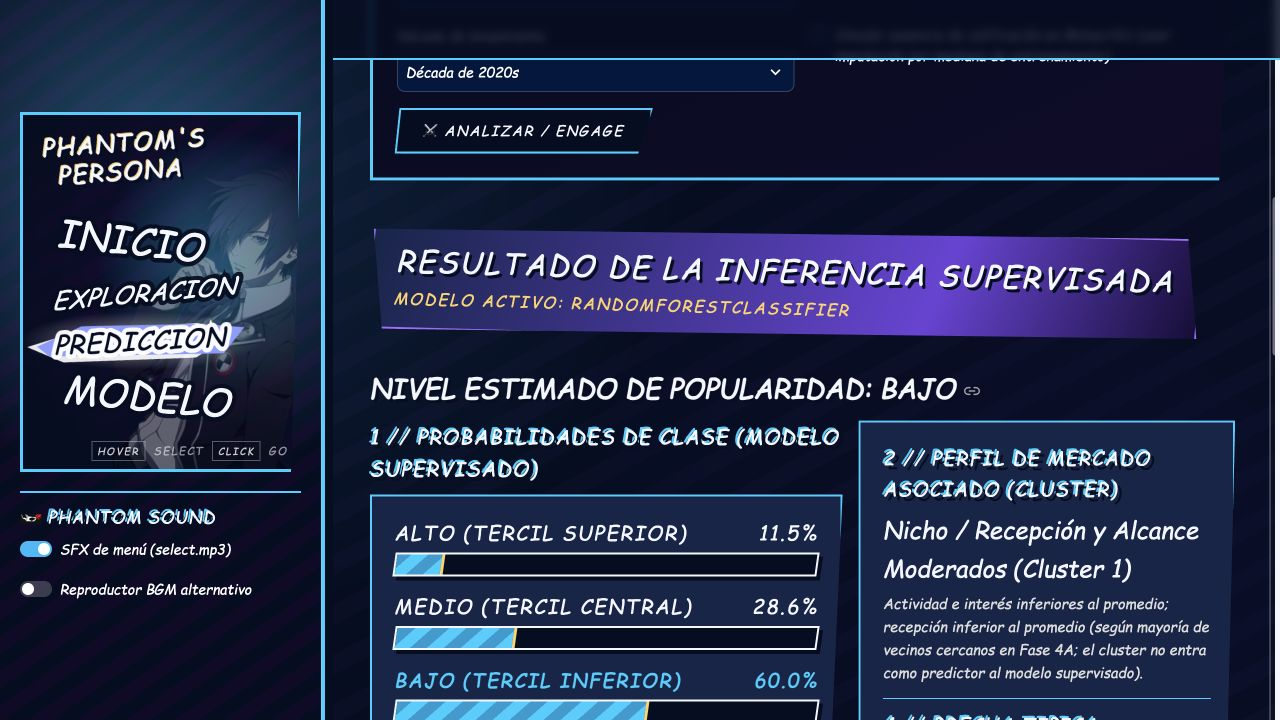
\includegraphics[width=\linewidth,height=.49\textheight,keepaspectratio]{figuras/escenario_S1.jpg}\caption{S1. Notas bajas: Rating 1.0 y prensa 45. Se muestra la clase baja como referencia del contraste.}\end{figure}\FloatBarrier
\begin{figure}[htbp]\centering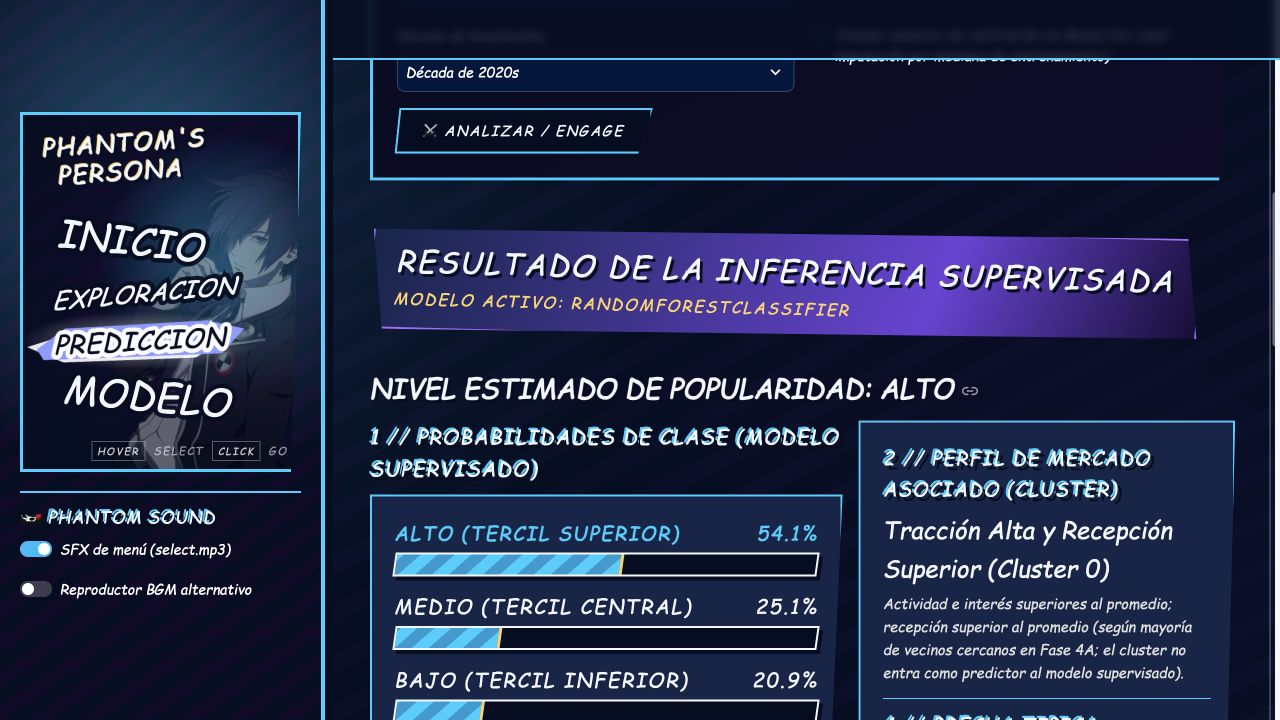
\includegraphics[width=\linewidth,height=.49\textheight,keepaspectratio]{figuras/escenario_S2.jpg}\caption{S2. Notas altas: Rating 4.8 y prensa 99. El resultado alto tiene una probabilidad de 54.1 por ciento.}\end{figure}\FloatBarrier
\begin{figure}[htbp]\centering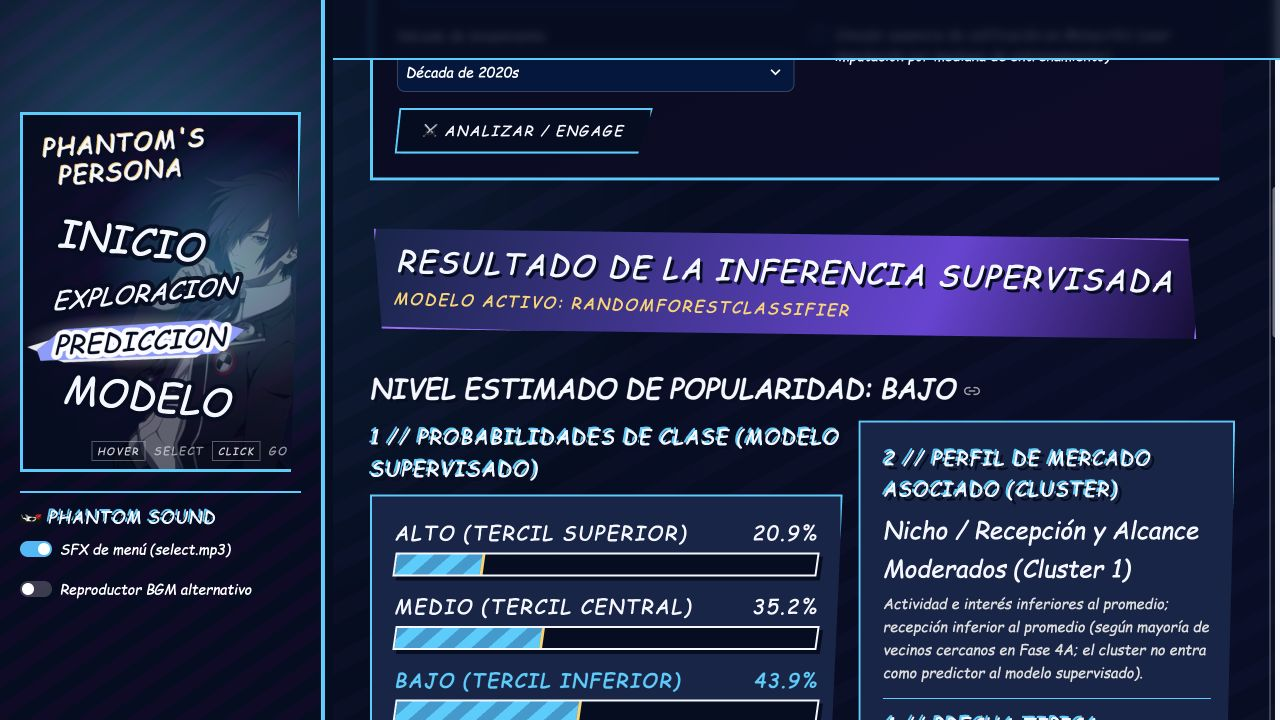
\includegraphics[width=\linewidth,height=.49\textheight,keepaspectratio]{figuras/escenario_S3.jpg}\caption{S3. Opiniones cruzadas: Rating 4.8 y prensa 45. El resultado bajo alcanza 43.9 por ciento.}\end{figure}\FloatBarrier
\begin{figure}[htbp]\centering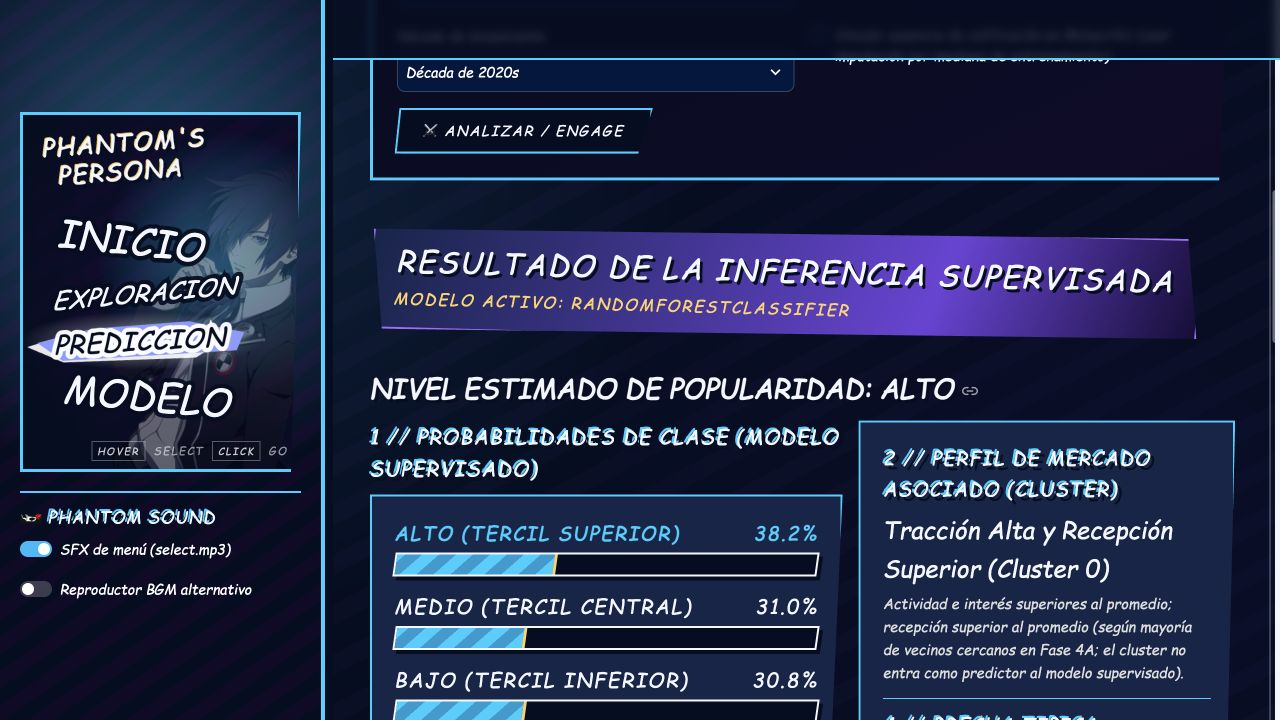
\includegraphics[width=\linewidth,height=.49\textheight,keepaspectratio]{figuras/escenario_S4.jpg}\caption{S4. Opiniones cruzadas: Rating 1.0 y prensa 99. Alto es la primera clase con 38.2 por ciento, sin mayoría absoluta.}\end{figure}\FloatBarrier
\begin{figure}[htbp]\centering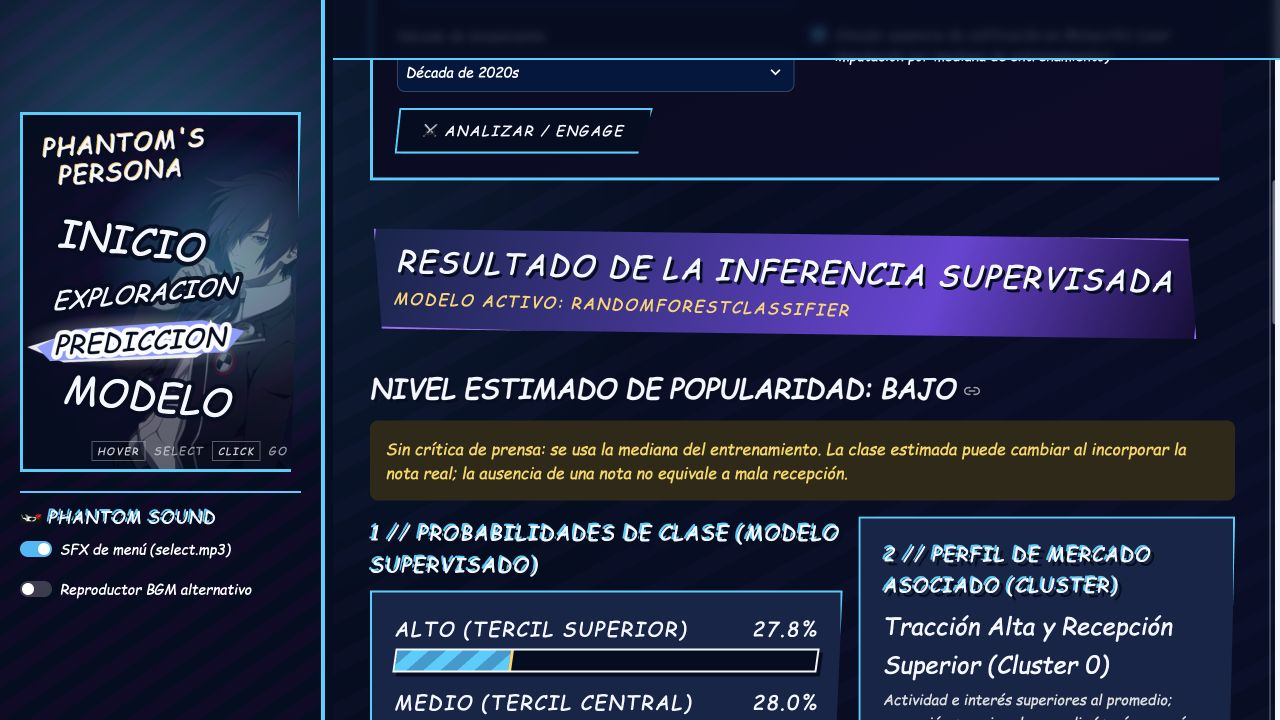
\includegraphics[width=\linewidth,height=.49\textheight,keepaspectratio]{figuras/escenario_S5.jpg}\caption{S5. Rating 4.8 y prensa ausente. El aviso explica la imputación; el perfil contextual no es la clase del clasificador.}\end{figure}\FloatBarrier
En S5 la pantalla puede mostrar una clase baja y un perfil contextual de tracción alta. No son dos respuestas del mismo clasificador: el perfil se adjunta desde los vecinos y sus clusters, mientras que la clase proviene del bosque. Que ambos utilicen atributos parecidos no convierte al perfil en una validación independiente de la predicción.
\subsection{Contraejemplos con juegos del conjunto de prueba}
Para no quedarnos solamente con escenarios inventados, seleccionamos un acierto y un error por cada clase real. Dentro de cada caso se tomó el registro con mayor probabilidad máxima del modelo. Esta selección es posterior a observar las predicciones y busca ilustrar sus límites; no sirve para estimar una nueva exactitud ni representa una muestra aleatoria de casos.
\begin{longtable}{p{.35\textwidth}p{.12\textwidth}p{.12\textwidth}p{.12\textwidth}p{.15\textwidth}}
\caption{Aciertos y errores reales frente al objetivo de popularidad del proyecto. No se usa ventas como verdad de referencia.}\\\hline
Juego&Clase real&Predicción&Resultado&Probabilidad\\\hline\endfirsthead
Juego&Clase real&Predicción&Resultado&Probabilidad\\\hline\endhead
Resident Evil 4: Wii Edition (ID 1335) & bajo & alto & Error & 66.8\%\\\hline
Pokémon Unite (ID 1054) & bajo & bajo & Acierto & 77.2\%\\\hline
Uncharted: The Nathan Drake Collection (ID 658) & medio & alto & Error & 69.8\%\\\hline
Pokémon Red (ID 1050) & medio & medio & Acierto & 52.0\%\\\hline
Jet Set Radio (ID 1057) & alto & bajo & Error & 49.2\%\\\hline
The Last of Us (ID 78) & alto & alto & Acierto & 82.4\%\\\hline
\end{longtable}
Uncharted: The Nathan Drake Collection es un contraejemplo importante. Su clase real es medio, pero el modelo lo coloca en alto con 69.8\,\%. Resident Evil 4: Wii Edition pertenece a bajo y también se estima alto, con 66.8\,\%. Estos casos refutan la idea de que una probabilidad elevada en la pantalla garantice que el modelo acertará. Por otro lado, The Last of Us sí se identifica como alto con 82.4\,\%; incluirlo muestra que tampoco sería correcto concluir, a partir de los errores, que el modelo nunca funciona.

Jet Set Radio permite ver el error en sentido contrario: su nivel real es alto y la estimación es bajo, con 49.2\,\%. La comparación se hace contra los terciles y la referencia de entrenamiento utilizados en el proyecto. Que un juego sea conocido fuera de Backloggd no cambia esa definición ni convierte la clasificación en un juicio sobre su calidad.

Para estos registros se conservaron ID, listas completas de género y organización, calificaciones, década, conteos y probabilidades. La comprobación numérica se hizo directamente con las entradas crudas del Pipeline. No se presenta una captura del formulario como réplica exacta de un registro con varias organizaciones o categorías que el formulario no permite seleccionar: esa distinción evita confundir una demostración simplificada con una reproducción del dato real.
\subsection{Cómo comprobamos la clase real de los ejemplos}
Los cortes de entrenamiento son 0.362294 y 0.626682. Bajo corresponde a un índice menor o igual al primer corte; medio supera el primero sin rebasar el segundo; alto supera el segundo. La tabla conserva los conteos y el índice calculado frente a esa referencia, no frente a una referencia ajustada con estos seis casos.
\begin{longtable}{p{.1\textwidth}p{.14\textwidth}p{.14\textwidth}p{.14\textwidth}p{.14\textwidth}p{.13\textwidth}}\caption{Señales observadas que permiten contrastar la clase real de los ejemplos. Los ID se corresponden con el archivo de evidencia.}\\\hline ID&Plays&Wishlist&Backlogs&Índice&Clase real\\\hline\endfirsthead ID&Plays&Wishlist&Backlogs&Índice&Clase real\\\hline\endhead
1335 & 1100 & 76 & 213 & 0.1327 & bajo\\\hline
1054 & 4500 & 65 & 184 & 0.2702 & bajo\\\hline
658 & 4300 & 319 & 1300 & 0.5708 & medio\\\hline
1050 & 8800 & 154 & 425 & 0.4482 & medio\\\hline
1057 & 3500 & 671 & 1900 & 0.6788 & alto\\\hline
78 & 17000 & 1400 & 2000 & 0.8959 & alto\\\hline
\end{longtable}
\subsection{Qué aprendimos de las pruebas}
Los escenarios permiten cuestionar dos expectativas del planteamiento inicial: una calificación alta no basta para asignar popularidad alta en todos los casos y una probabilidad mayor tampoco garantiza una predicción correcta. La ausencia de prensa, el género y la organización cambian el espacio de entrada, mientras que la clase real depende de actividad e interés observados que deliberadamente no se entregan como predictores.

Por eso la aplicación debe entenderse como una estimación orientativa que ayuda a contrastar situaciones. Los contraejemplos no se utilizaron para volver a escoger parámetros sobre la prueba. La forma adecuada de evaluar una mejora futura sería reservar una muestra temporal nueva y establecer antes los criterios de comparación. Reentrenar hasta que desaparezcan estos seis errores solo memorizaría una parte de la evaluación que ya conocemos.

\section{Plan real frente a la línea base}\label{sec:plan}
La línea base del anteproyecto v2.0 programaba actividades del 1 de octubre al 25 de noviembre de 2026. El equipo declara que las actividades técnicas realizadas cumplieron el calendario previsto. La tabla contrasta ese plan con los productos disponibles y las desviaciones de alcance documentadas. No se asignan fechas exactas de terminación porque no se cuenta con un registro por actividad; la entrega y exposición académicas se distinguen de la ejecución técnica.
\begin{longtable}{p{.22\textwidth}p{.19\textwidth}p{.49\textwidth}}
\caption{Línea base frente a evidencia disponible al 9 de noviembre de 2026.}\\\toprule Actividad & Línea base & Estado real y justificación\\\midrule\endfirsthead
Actividad&Línea base&Estado real y justificación\\\midrule\endhead
Anteproyecto y revisión & 1--5 octubre & Documento v2.0 conservado como antecedente; auditorías posteriores revisaron su alcance. No se reconstruye su fecha de terminación.\\
Limpieza y validación & 6--15 octubre & Scripts, dataset y log disponibles. Se recibe un maestro ya curado y se auditan decisiones heredadas.\\
EDA y correlaciones & 15--29 octubre & Tablas y figuras ejecutadas. Se distingue asociación de brecha y se exige cobertura mínima por grupo.\\
Clustering e interpretación & 29 octubre--10 noviembre & K-Means y DBSCAN ejecutados en Python y Weka; DBSCAN no produjo varios perfiles útiles.\\
Clasificación & 5--11 noviembre & Cuatro familias de producción evaluadas. Se reemplazó la comparación MLP prevista por bosque; no hay resultado MLP.\\
Arquitectura y web & 8--16 noviembre & Web funcional comprobada al corte, anterior al fin planeado; no se atribuyen horas de adelanto sin bitácora temporal completa.\\
Despliegue público & 16--18 noviembre & Cancelado por preferencia de mantener datos y modelos locales; demo en localhost.\\
Evaluación en Orange & Durante modelado & Descartada por cierres; Weka sí conserva seis corridas gráficas.\\
Documento y revisión & 10--24 noviembre & Integración al corte actual con evidencia y bibliografía. No se afirma entrega formal al profesor.\\
Entrega y demo & 25 noviembre & Fecha planificada; ejecución local verificada, presentación académica aún no acreditada.\\\bottomrule
\end{longtable}
Las principales desviaciones no fueron simples cambios de calendario: se sustituyó el target de perfil de cluster por terciles de popularidad, se corrigió la procedencia de notas y se recalculó el objetivo dentro de la validación. También se abandonó Orange y se mantuvo la app local. Estos ajustes reducen el alcance respecto de promesas iniciales, pero hacen que lo reportado sea comprobable.
\section{Evaluación de los objetivos y discusión}\label{sec:discusion}
El objetivo de inspección se cumple con un esquema comprobado, log de preparación, pruebas y conservación del maestro. La existencia de tres conflictos históricos impide afirmar que todos los registros tengan verificación semántica externa. Se conserva esa incertidumbre en la elegibilidad en vez de escoger el máximo o promediar variantes de forma arbitraria.

El objetivo de relaciones se cumple con Pearson, Spearman, tamaños y p-valores segmentados. La hipótesis de coincidencia perfecta entre comunidad y prensa no se sostiene. Tampoco puede concluirse que un género sea mejor oportunidad comercial por su correlación o por su brecha media: esas medidas no evalúan demanda no satisfecha, competencia ni ingresos.

En la parte de agrupamiento se obtuvieron dos perfiles con K-Means que permiten resumir diferencias de actividad, interés y recepción. Sin embargo, DBSCAN no encontró varios segmentos útiles con la configuración establecida. Esto también forma parte del resultado: el hecho de aplicar un algoritmo no obliga a que aparezcan los grupos que esperábamos. Los nombres de los perfiles se utilizaron para explicar sus promedios y no para afirmar que todo el mercado se divide de esa manera.

El clasificador supera a la referencia en la partición disponible, pero sigue confundiendo especialmente la clase media. Su etiqueta es un tercil artificial y depende de una referencia histórica del catálogo. Una predicción no puede comprobarse contra ventas ni contra el futuro solo porque el formulario funcione; son validaciones distintas.

La propuesta propia integra control de procedencia, objetivo local, agrupación por título, inferencia cruda y pruebas de interfaz. Esto aporta trazabilidad respecto de una corrida aislada. Aun así, la CV no anidada y la ausencia de validación externa limitan cualquier comparación predictiva más fuerte.
\section{Conclusiones}\label{sec:conclusiones}
Después de realizar el análisis, podemos concluir que la idea inicial de revisar varios indicadores sí fue útil. Las calificaciones nos ayudaron a entender la recepción, mientras que Plays, Backlogs y Wishlist mostraron diferencias de alcance e interés que no se veían solamente con una nota. La relación entre usuarios y prensa fue positiva, aunque moderada, por lo que tampoco sería correcto asumir que ambas opiniones siempre coinciden.

K-Means ofrece una síntesis interpretable de dos niveles conjuntos de actividad y recepción, pero no demuestra mercados naturales. DBSCAN no generó una segmentación múltiple útil bajo el protocolo fijado. Conservar ese resultado, y la diferencia de ruido entre Weka y Python, permite explicar lo que cada herramienta produjo sin acomodarlo a una expectativa.

En cuanto a la predicción, sí se logró construir un modelo que supera a la referencia mayoritaria, pero los resultados no permiten decir que pueda decidir por sí solo qué videojuego tendrá éxito. La clase media siguió siendo difícil y los escenarios mostraron que algunas respuestas cambian bastante cuando falta la nota de prensa. También se entrenaron siete variantes adicionales del bosque y ninguna mejoró el criterio de validación utilizado. Por eso se conservó el modelo que ya teníamos, en lugar de presentar como mejora un cambio que no estaba respaldado por sus resultados.

La web convierte el análisis en una demostración consultable y mantiene visibles los límites de las estimaciones. La ausencia de Metacritic puede alterar mucho una respuesta y requiere cautela. Para estudiar nuevos lanzamientos o rentabilidad necesitaríamos una muestra temporal externa, métricas comerciales observadas, control de plataforma y fecha, y un diseño específico para esa pregunta.

Por tanto, resolvemos la exploración de recepción y popularidad relativa dentro del catálogo y entregamos una herramienta local verificable. No demostramos reducción de pérdidas ni capacidad para anticipar éxito comercial de juegos como servicio. La conclusión se limita deliberadamente a la evidencia que tenemos.
\section{Reproducibilidad y alcance de la verificación}
El repositorio organiza original en data/raw, derivados en data/clean, código en src, artefactos en models, pruebas en tests y evidencias en reports. Los scripts usan pathlib y semilla 42 cuando el método dispone de aleatoriedad. La carpeta de este documento copia figuras y tablas para poder compilar sin rutas absolutas ni conexión a los directorios originales.

Se aprobaron 101 pruebas en la ejecución completa más reciente de la suite; la revisión específica anterior de inferencia, modelo, pipeline y visualización incluyó 39 pruebas. Las 222 predicciones almacenadas coinciden con el artefacto; las probabilidades son válidas y los vecinos contienen solo IDs de entrenamiento en el mismo espacio. Veinte archivos de datos y modelos conservaron sus hashes durante esa revisión. Esto comprueba integridad e implementación, no la verdad externa de cada calificación.

El informe se puede compilar con \texttt{latexmk -pdf main.tex}. El manifiesto local identifica hashes de las evidencias copiadas. La bibliografía distingue documentos metodológicos y fuentes de software de las mediciones propias del proyecto. La consulta al sitio de Kaggle confirma su identificación, pero no sustituye el archivo local por una versión actual del servicio.

La documentación y el código recibieron apoyo de asistentes de inteligencia artificial, incluidas operaciones gráficas autorizadas y revisión automatizada. Los resultados se verificaron contra archivos y pruebas; no se presenta esa asistencia como validación humana independiente de cada dato. La responsabilidad académica y la aprobación final corresponden al equipo autor.
\appendix
\section{Correspondencia con la rúbrica}
\begin{longtable}{p{.25\textwidth}p{.65\textwidth}}\toprule Rubro& Evidencia en el documento\\\midrule
Objetivo & Sección~\ref{sec:objetivos}: objetivo general delimitado y seis objetivos verificables.\\
Contexto & Sección~\ref{sec:contexto}: origen, maestro curado, unidad analítica, escalas y sesgos.\\
Estrategia & Sección~\ref{sec:estrategia}: CRISP-DM y función de herramientas.\\
Expectativas & Sección~\ref{sec:objetivos}: criterios comprobables y alcance excluido.\\
Plan baseline y real & Sección~\ref{sec:plan}: ventanas originales, evidencia al corte y desviaciones.\\
Metodología & Secciones~\ref{sec:preparacion}--\ref{sec:clasificacion}: preparación, relaciones, clustering y clasificación.\\
Herramientas y propuesta & Secciones~\ref{sec:clasificacion}--\ref{sec:web}: Python, corridas Weka y demo local; Orange sin resultados.\\
Resultados y conclusiones & Secciones~\ref{sec:eda}--\ref{sec:weka} y \ref{sec:discusion}--\ref{sec:conclusiones}: resultados positivos, negativos y límites.\\
Fuentes & Bibliografía APA y referencias internas a evidencias.\\\bottomrule\end{longtable}
\section{Guion reproducible de la demostración}
\begin{enumerate}
\item Abrir Inicio y explicar que el maestro tiene 1,117 registros y el antecedente 1,512; mostrar la limitación de ventas.
\item En Exploración, cambiar Plays a Wishlist y distinguir asociación de brecha. Identificar el tamaño de pares del grupo consultado.
\item En Modelo, leer la matriz: medio tiene 27 aciertos de 80. Explicar por qué esto limita una exactitud global moderada.
\item En Predicción, seleccionar Adventure y RPG, organización Otro, década 2020, Rating cinco y Metacritic cien. La evidencia guardada muestra alto con 54.1\,\%.
\item Ocultar Metacritic y enviar de nuevo: bajo con 44.2\,\%. Mostrar el aviso y explicar sensibilidad, imputación y probabilidades sin calibrar.
\item Abrir las capturas originales de Weka y contrastar 892 casos de CV con 222 de prueba de producción. No atribuir silhouette de Python ni resultados a Orange.
\end{enumerate}
\section{Fuentes locales y trazabilidad}
La inspección y limpieza están en reports/inspeccion.md y limpieza\_log.md. Las relaciones, perfiles y sensibilidad se conservan en reports/clustering.md y sus CSV. Las métricas de producción están en models/metadata.json y reports/modelo\_comparacion.csv. El contraste entre herramientas está en reports/tables/comparativo\_herramientas.csv. Las seis corridas y capturas están en reports/weka y su respaldo ZIP verificado. La revisión adicional de predicción se conserva en reports/revision\_predicciones, incluyendo auditoria.json, decision.json y la bitácora unificada de esa carpeta.

Los nombres completos se conservan en el manifiesto y las tablas copiadas. No se atribuyen nuevas corridas a las capturas históricas. El PDF de criterios del profesor se adjunta como evidencia/rubrica\_proyecto.pdf y se utiliza como guía de cobertura, no como fuente de mediciones.
\section{Capturas actuales de la aplicación}
Las siguientes capturas se tomaron durante la integración de este documento, tras iniciar el servidor local. Se distinguen de las evidencias históricas de Weka y de los casos de predicción ya verificados. Weka permaneció cerrado.
\begin{figure}[htbp]\centering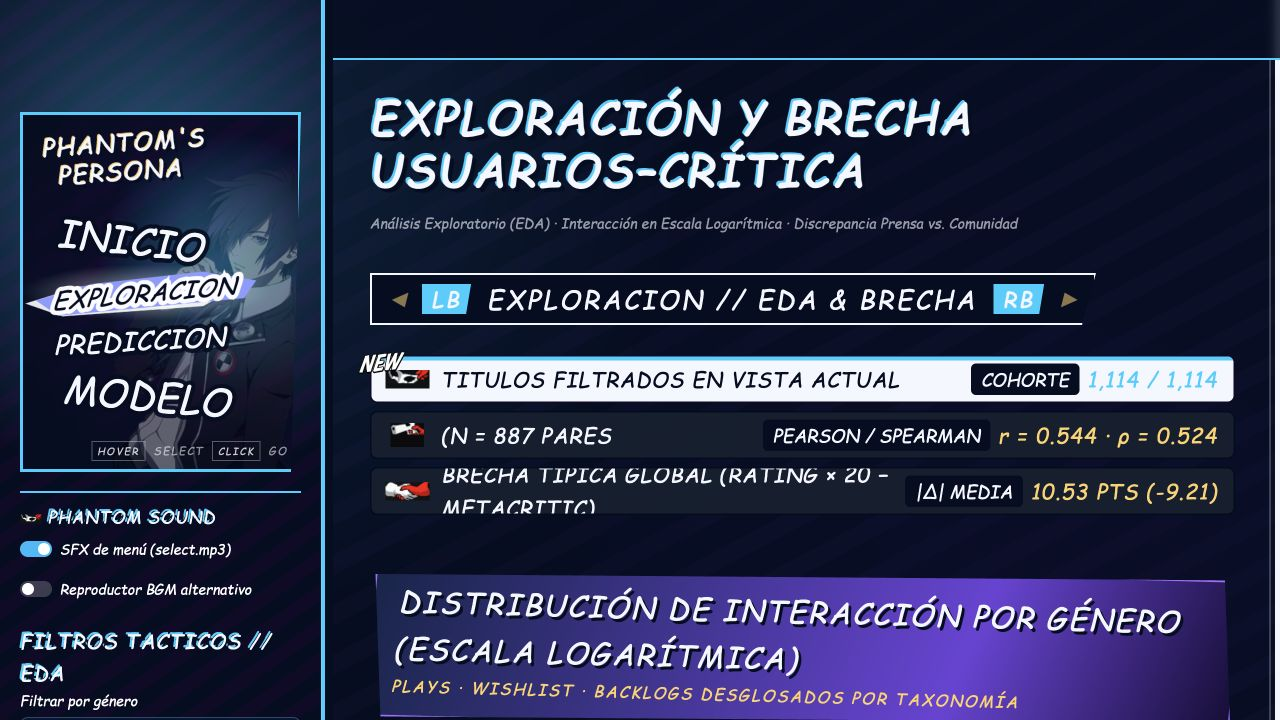
\includegraphics[width=\linewidth]{figuras/exploracion_actual.jpg}\caption{Página Exploración capturada al corte documental.}\end{figure}\FloatBarrier
\begin{figure}[htbp]\centering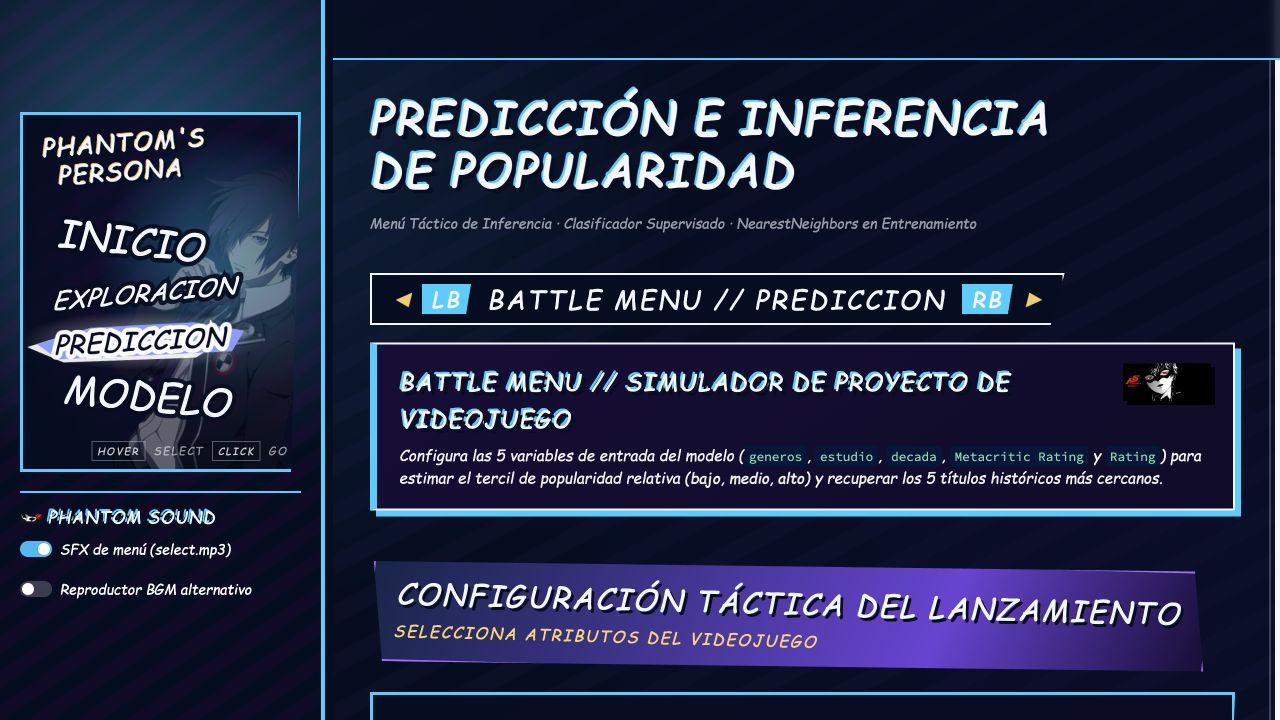
\includegraphics[width=\linewidth]{figuras/prediccion_actual.jpg}\caption{Página Predicción y acceso al formulario crudo.}\end{figure}\FloatBarrier
\begin{figure}[htbp]\centering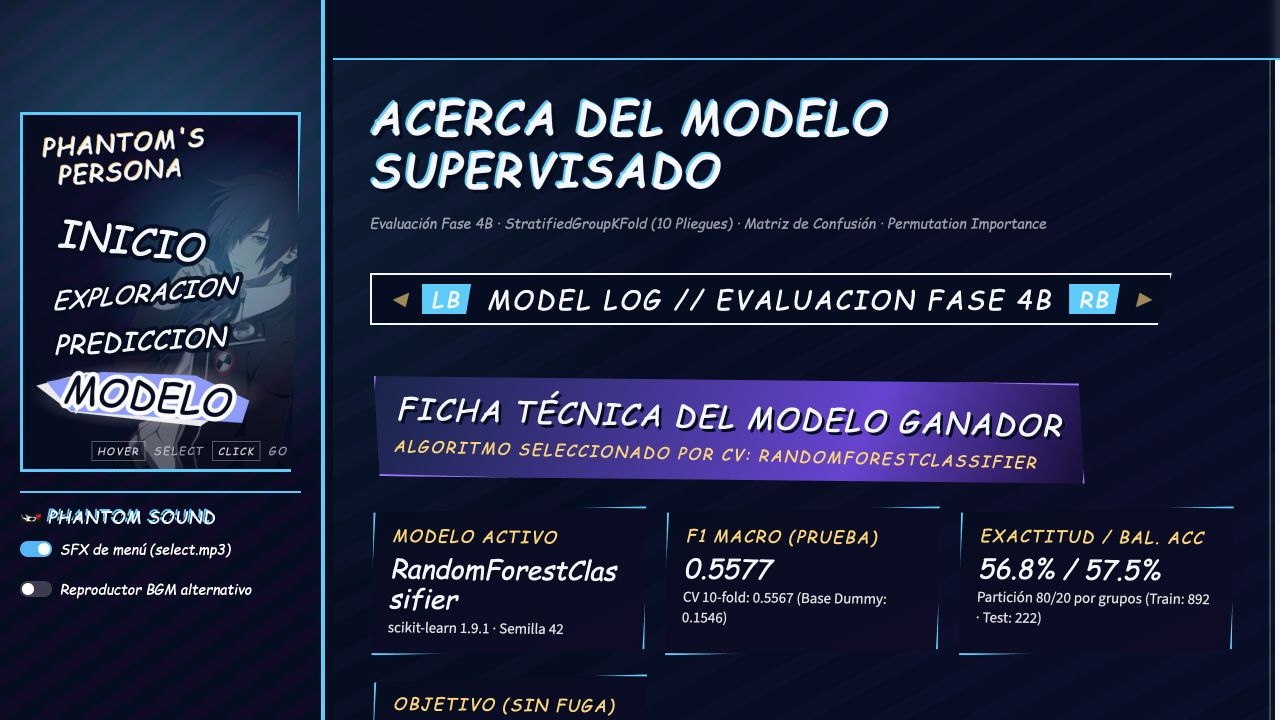
\includegraphics[width=\linewidth]{figuras/modelo_actual.jpg}\caption{Página Modelo con métricas del artefacto vigente.}\end{figure}\FloatBarrier
\nocite{chaki2023popular,chapman2000crisp,pedregosa2011scikit,mckinney2010pandas,frank2016weka,ester1996dbscan}
\clearpage\pagestyle{referencias}\printbibliography[heading=bibintoc,title={Referencias}]
\end{document}
